\documentclass[letterpaper,onecolumn,10pt,journal,final]{IEEEtran}

\usepackage{latexsym}


\usepackage[spanish,es-tabla]{babel}

\usepackage{amsmath}

\makeatletter
\newcommand\xleftrightarrow[2][]{%
  \ext@arrow 9999{\longleftrightarrowfill@}{#1}{#2}}
\newcommand\longleftrightarrowfill@{%
  \arrowfill@\leftarrow\relbar\rightarrow}
\makeatother

\usepackage{amsfonts}
\usepackage{subfigure}
\usepackage{psfrag}
\usepackage{colortbl}
\usepackage{color}
\usepackage[sectionbib]{chapterbib}
\usepackage{afterpage}
\usepackage{booktabs}

\usepackage{graphicx}
\usepackage{url}
\usepackage{amsmath}
\interdisplaylinepenalty=2500
\usepackage[english]{babel}
%\usepackage{array,booktabs,arydshln,xcolor}
\usepackage{flushend}
\hyphenation{industrial electronics IEEEtran}
\usepackage[font=footnotesize,caption=false,farskip=0mm,captionskip=0mm,nearskip=0mm]{subfig}
\usepackage{cite}
\usepackage{amsmath}
\usepackage{array}
\usepackage{graphicx}
\usepackage{latexsym}
\usepackage{psfrag}
\usepackage{color}
\usepackage{multirow}
\usepackage{stfloats}
\usepackage{enumerate}
% Paquetes adicionales para insertar código con formato m-file de MATLAB
\usepackage{listings}   % Permite incorporar código con diferentes formatos
\usepackage{float}
%usepackage{caption}
\usepackage[font=bf]{caption}
% falta cambiar el font size de caption  a 9pt
\usepackage[dvips]{graphicx}
\usepackage[framed,numbered,final]{mcode}% Configura listings para que el resultado se vea igual al editor de MATLAB
\usepackage{xcolor}
\usepackage{textcomp}

%\usepackage [latin1]{inputenc}
%\renewcommand\lstlistingname{Code}% Cambia el nombre del objeto listings

%ejemplo matlab code:

%\begin{lstlisting}[frame=single]
%a = 15;				% Por defecto es tipo 'double'
%b = uint8(a);		
%c = int16(32767);
%\end{lstlisting}

\parskip 0pt

\usepackage{lipsum}

\newcommand\blfootnote[1]{%
  \begingroup
  \renewcommand\thefootnote{}\footnote{#1}%
  \addtocounter{footnote}{-1}%
  \endgroup
}

\begin{document}
\title{ELO 314 - Procesamiento Digital de Señales\\ Laboratorio 4: Transformada Discreta de Fourier en MatLab}

\author{\textbf{Preparado por}
\vspace{1 mm}Juan Aguilera e-mail: Juan.Aguileraca@sansano.usm.cl \\
            Cristóbal Huidobro e-mail: 
cristobal.huidobro@sansano.usm.cl}

\maketitle

\vspace{-1 cm}

%\setcounter{section}{0}
%%%%%%%%%%%%%%%%%%%%%%%%%%%%%%%%%%%%%%%%%%%%%%%%%%%%%%%%%%%%%%%%%%%%%%%%%%%%%%%%%
%
%-----I C ́ALCULO DE LADFTPARASE ̃NALESSIMPLES---------------------------------%
%
%%%%%%%%%%%%%%%%%%%%%%%%%%%%%%%%%%%%%%%%%%%%%%%%%%%%%%%%%%%%%%%%%%%%%%%%%%%%%%%%%
\section{Cálculo de la DFT para señales simples}
\begin{enumerate}[1)]
    \item %1)-------------------------------------------------------------------------% 
    
Para el calculo de la expresión analítica tenemos que
\begin{equation*}
    \omega _0 = \frac{2 \pi f}{f_s} = \frac{2 \pi \cdot 100}{5000} [rad/muestra]
\end{equation*}
Por lo que las señales quedan expresadas de la siguiente manera:
\begin{itemize}
    \item $x_1 [n] = sin[ \omega _0 n] = \frac{e ^{j \omega _0 n}-e ^{-j \omega _0 n} }{2j}$
    \item $x_2 [n] = cos[ \omega _0 n] = \frac{e ^{j \omega _0 n}+ e ^{-j \omega _0 n} }{2}$
\end{itemize}
Por lo que la DTFT de la señal $x_1[n]$ se calcula de la siguiente manera:
\begin{equation*}
    \begin{split}
    X_1(\omega ) &= \frac{1}{2j} \sum _{n=- \infty } ^{ \infty} \left( e ^{j \omega _0 n}-e ^{-j \omega _0 n} \right)  e^{-j \omega n} \\
    \Rightarrow & \frac{1}{2j} \sum _{n=- \infty } ^{ \infty} \left( e ^{ - j n( \omega - \omega _0)}-e ^{- j n( \omega + \omega _0)} \right) \\
    \Rightarrow & \frac{2 \pi }{2 j} \left( \delta (\omega -  \omega _0) - \delta (\omega + \omega _0 )  \right)\\
    \Rightarrow & \frac{2 \pi j }{2} \left( \delta (\omega +  \omega _0) - \delta (\omega - \omega _0 )  \right), ~~~~ \omega \in [0,2 \pi)
    \end{split}
\end{equation*}

De forma similar, para $x_2[n]$ tenemos:
\begin{equation*}
    \begin{split}
    X_2(\omega ) &= \frac{1}{2} \sum _{n=- \infty } ^{ \infty} \left( e ^{j \omega _0 n}+e ^{-j \omega _0 n} \right)  e^{-j \omega n} \\
    \Rightarrow & \frac{1}{2} \sum _{n=- \infty } ^{ \infty} \left( e ^{ - j n( \omega - \omega _0)}+e ^{- j n( \omega + \omega _0)} \right) \\
    \Rightarrow & \frac{2 \pi }{2} \left( \delta (\omega -  \omega _0) + \delta (\omega + \omega _0 )  \right), ~~~~ \omega \in [0,2 \pi)
    \end{split}
\end{equation*}

Asumiendo la duración real de la señal tenemos para $x_1[n]$:
\begin{equation*}
    \begin{split}
    X_1(\omega ) &= \frac{1}{2j} \sum _{n= 0 } ^{ 500} \left( e ^{j \omega _0 n}-e ^{-j \omega _0 n} \right)  e^{-j \omega n} \\
    \Rightarrow & \frac{1}{2j} \sum _{n= 0 } ^{ 500} \left( e ^{ - j n( \omega - \omega _0)}-e ^{- j n( \omega + \omega _0)} \right) \\
    \Rightarrow & X_1 ( \omega ) = 
  \begin{cases} 
   -250j & \text{si } \omega = \omega _0 \\
   250j  & \text{si } \omega = - \omega _0\\
   0 & e.o.c
  \end{cases}
    \end{split}
\end{equation*}

De forma similar, para $x_2[n]$ tenemos que:
\begin{equation*}
    \begin{split}
    X_2(\omega ) &= \frac{1}{2} \sum  _{n= 0 } ^{ 500}  \left( e ^{j \omega _0 n}+e ^{-j \omega _0 n} \right)  e^{-j \omega n} \\
    \Rightarrow & \frac{1}{2} \sum _{n= 0 } ^{ 500}  \left( e ^{ - j n( \omega - \omega _0)}+e ^{- j n( \omega + \omega _0)} \right) \\
    \Rightarrow & X_2 ( \omega ) = 
  \begin{cases} 
   250 & \text{si } \omega = \pm \omega _0 \\
   0 & e.o.c
  \end{cases}
    \end{split}
\end{equation*}

Como consecuencia de tomar la duración real de la señal, la DTFT depende de un factor que depende de el numero de muestras.
% no se si sea necesario hacer calculos o explicaciónes adicionales, no se me da mucho eso ajaja.


    \item %2)-------------------------------------------------------------------------%
 
Se aplica el comando de $MATLAB$ $fft$, obteniendo como resultado% lo siguiente. 
%\begin{enumerate}
%    \item 
%    \item
%\end{enumerate}
lo que se aprecia en la Figura \ref{fig:I2}.
\begin{figure}[H]
\centering
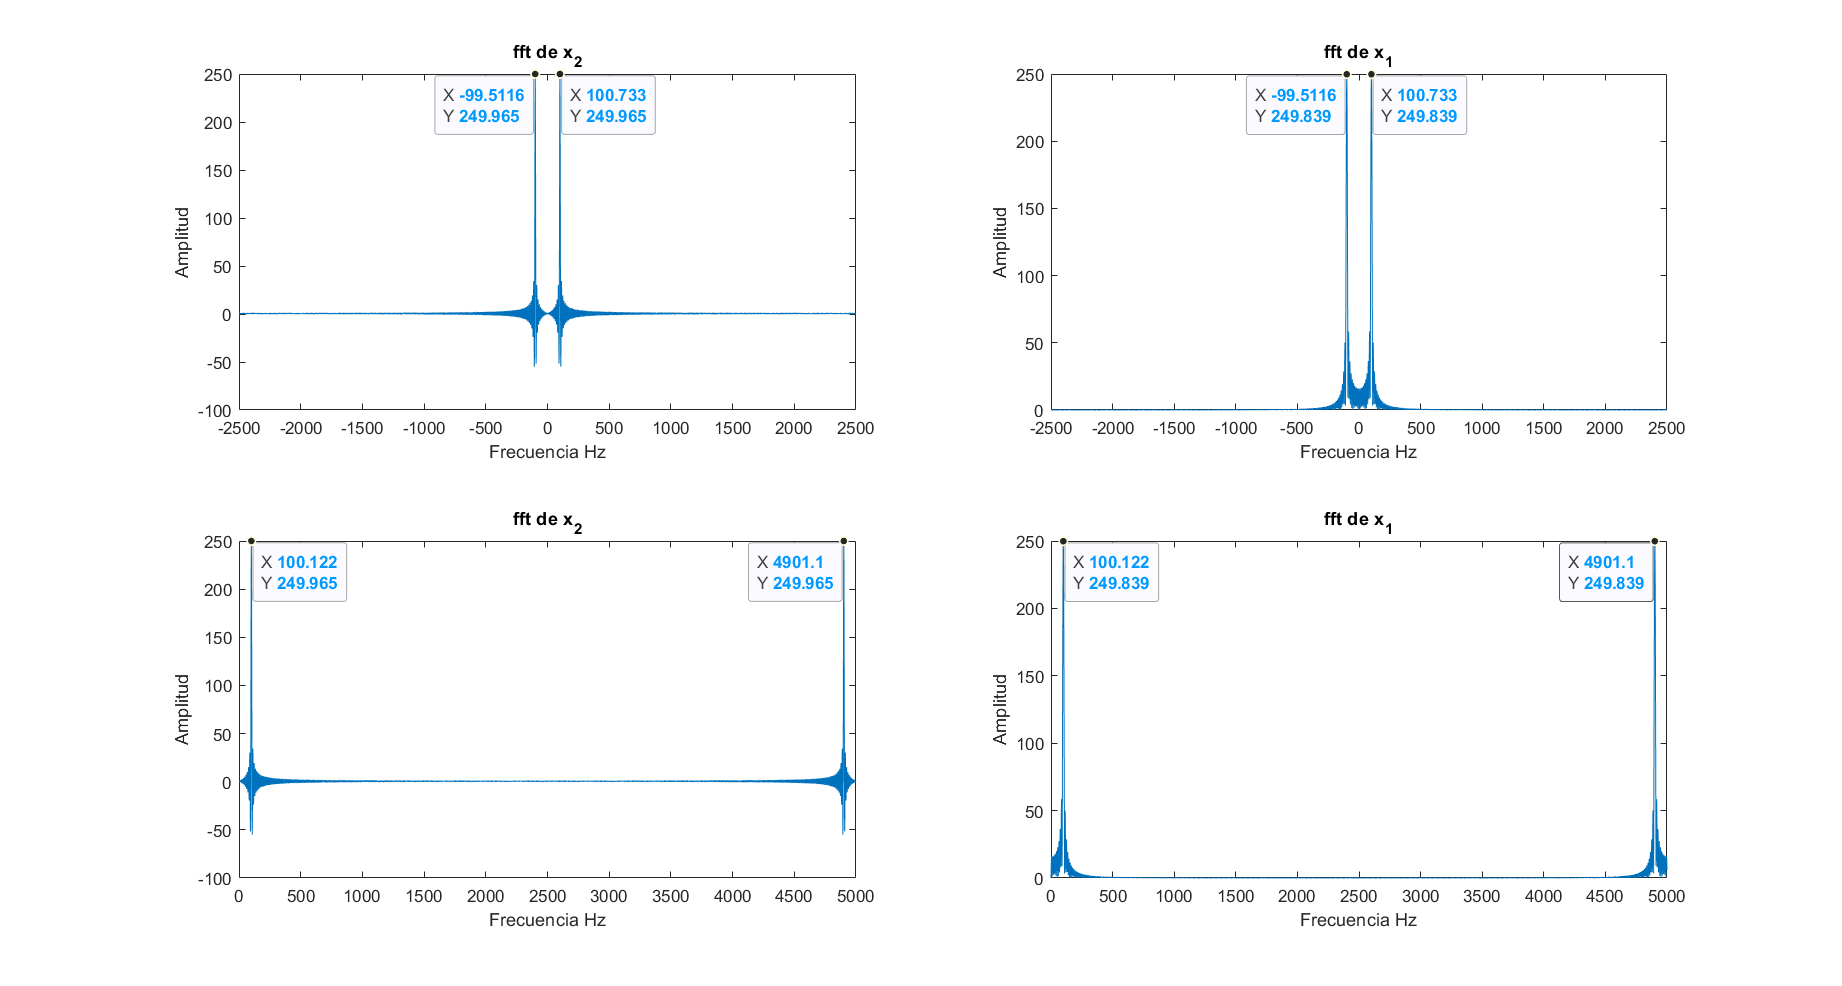
\includegraphics[width=1 \linewidth]{Figuras/I2)a.png}
\caption{fft de señales $x_1$ y $x_2$ para diferentes intervalos de frecuencia.}
\label{fig:I2}
\end{figure}

La magnitud esperada, correspondiente a la suma de los puntos donde $\omega = \pm \omega _0$, es de 250. Se esperaría que para una señal de tiempo infinito, el resultado de la DTFT se comporte como un delta, es decir, que tenga amplitud infinita en los puntos donde $\omega = \pm \omega _0$. A pesar de aumentar el numero de muestras a $N = 4069$, la amplitud en  $\omega = \pm \omega _0$ no debería aumentar en más de 250 unidades, esto debido a que la señal utilizada solo tiene un largo de 500 muestras, por lo que, aunque se aumenten las muestras totales, solo 500 de ellas sumaran en la amplitud de los deltas.

Sin embargo se observa que la magnitud es un poco menor a 250, además de presencia de energía en los valores que rodean a $\omega_0$. Esto se debe a que como la señal es de menor largo que el numero de muestras requeridas para la DFT, esta rellena las muestras restantes con $0$, lo que sería equivalente a enventanar la señal con una ventana cuadrada.

% no se redactar.
\newpage

    \item %3)-------------------------------------------------------------------------%
Los valores de magnitud, parte real e imaginara vs frecuencias se muestran a continuación.
\begin{enumerate}
    \item Magnitud vs Frecuencia
\begin{figure}[H]
\centering
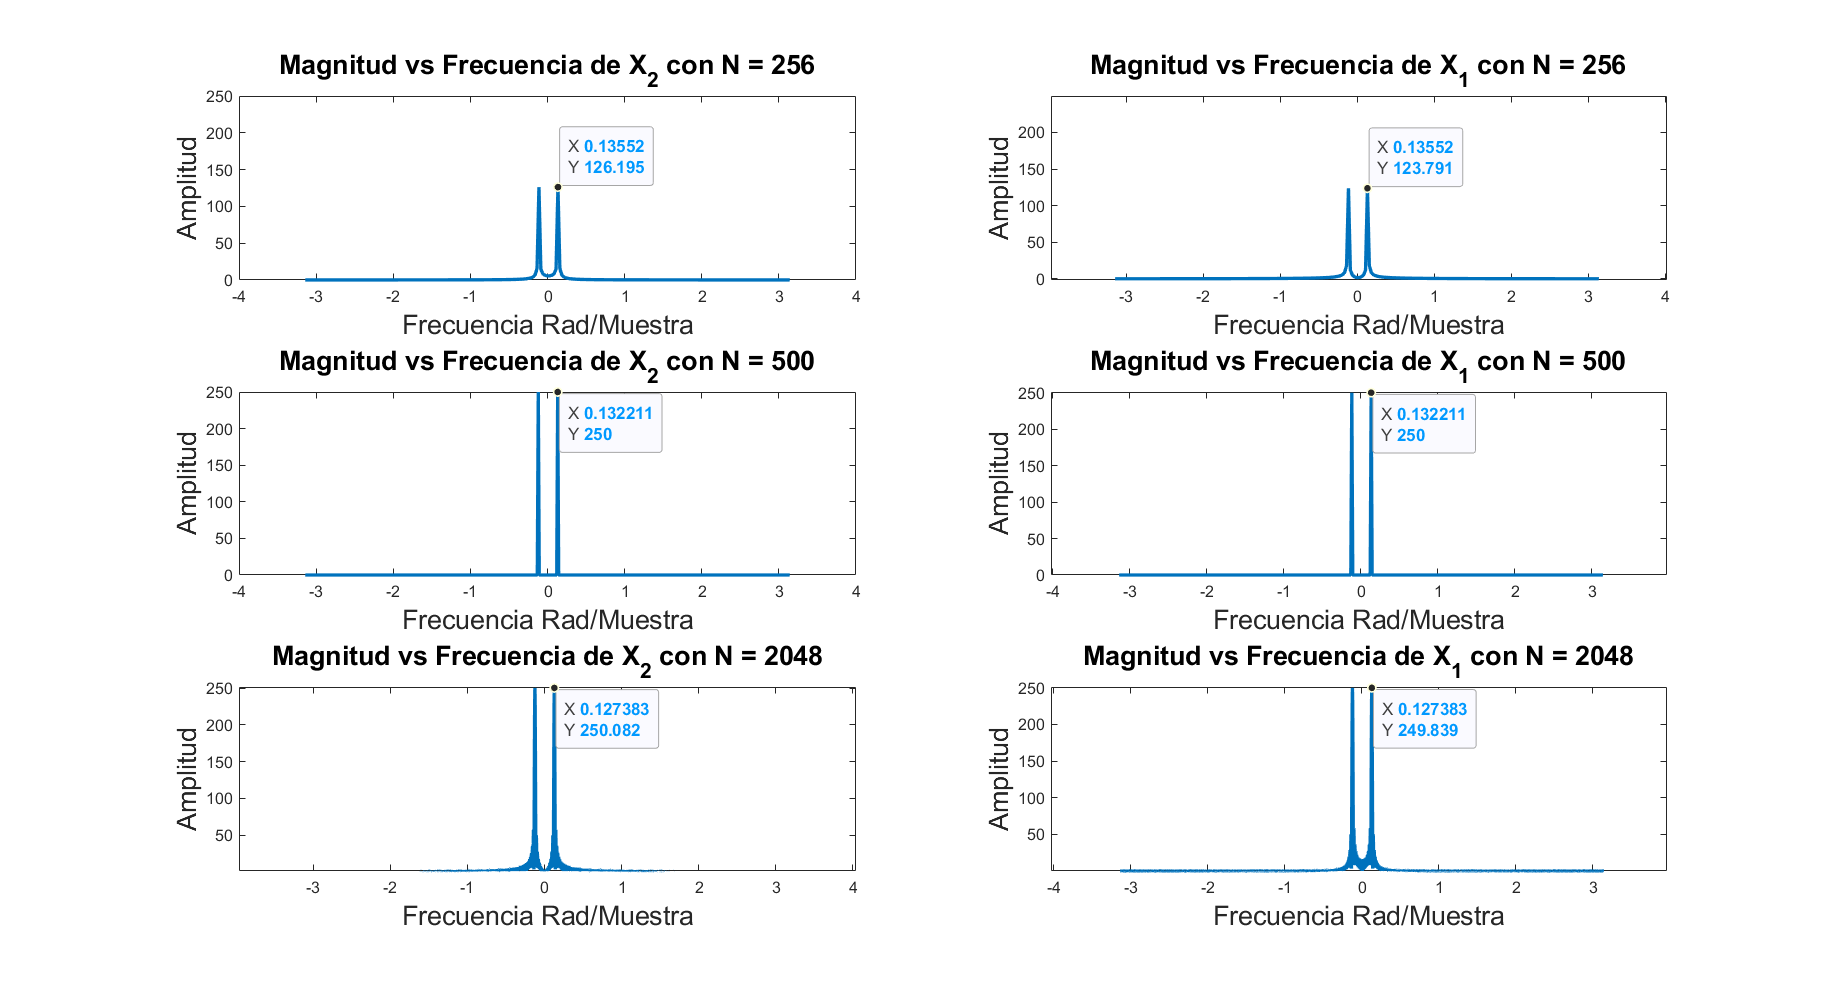
\includegraphics[width=1 \linewidth]{Figuras/I3)a.png}
\caption{Magnitud vs Frecuencia para diferentes valores de N.}
\label{fig:I3)a}
\end{figure}
    
    \item Parte Real vs Frecuencia
    
\begin{figure}[H]
\centering
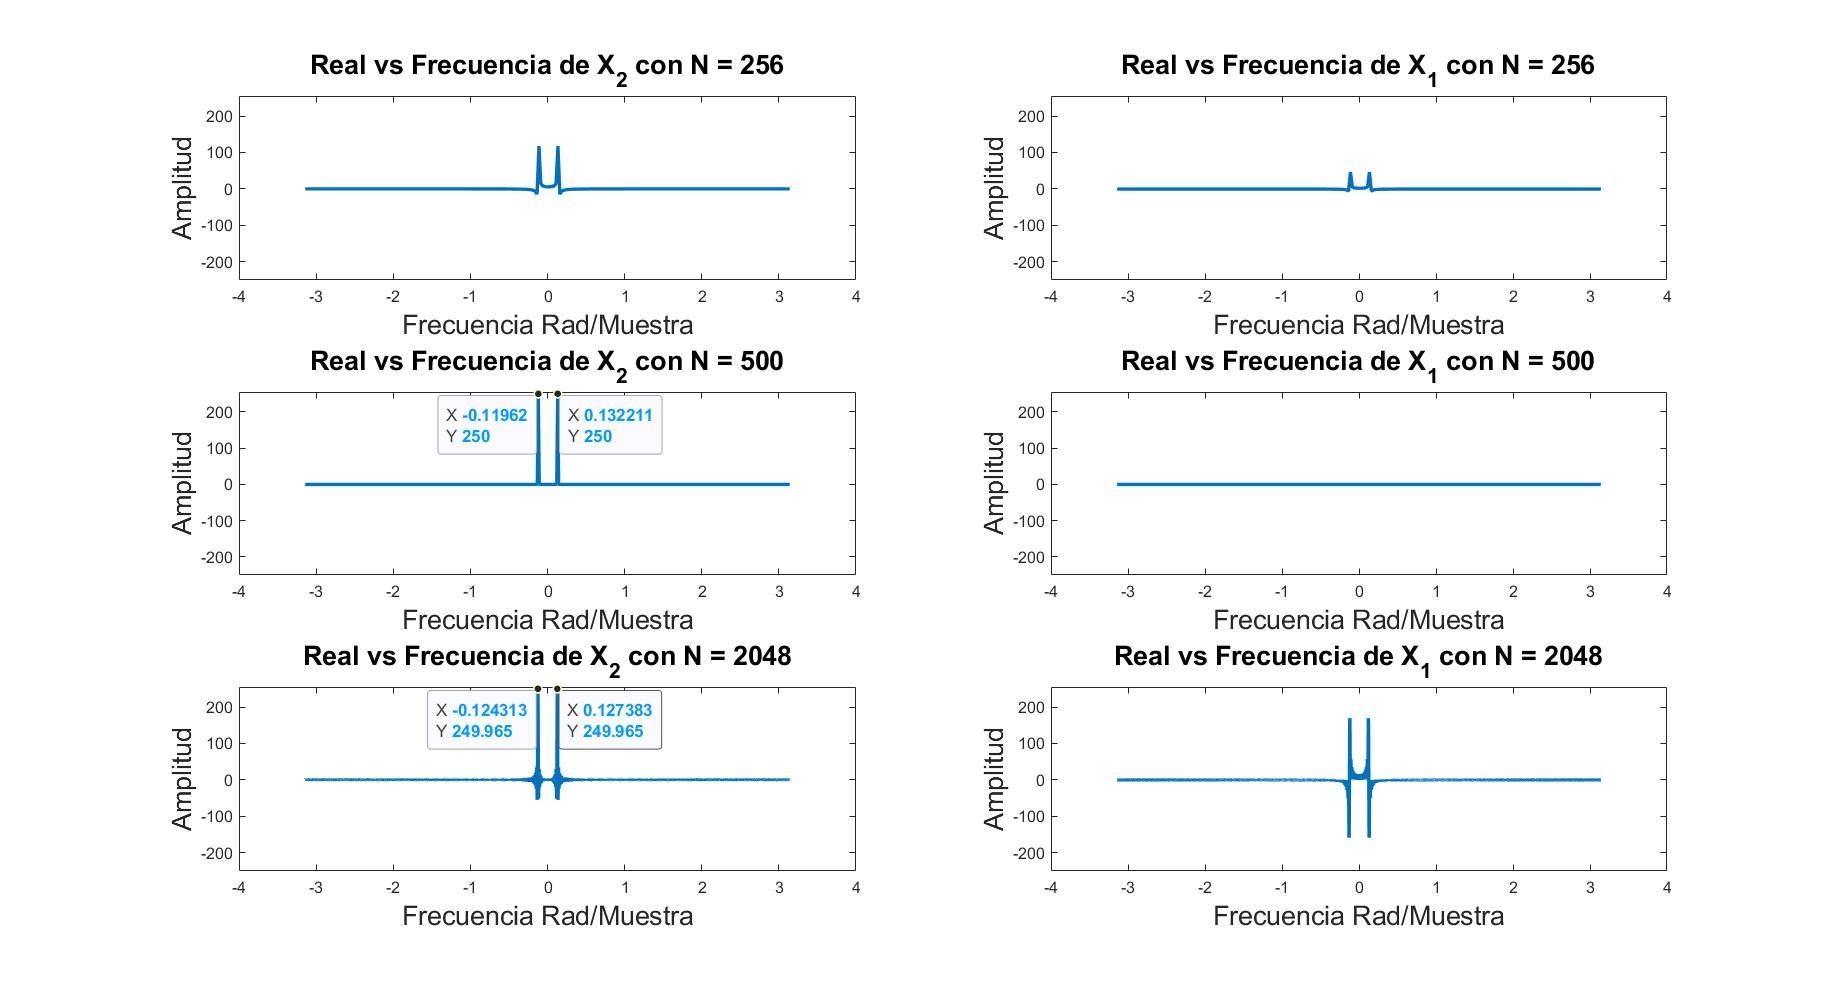
\includegraphics[width=1 \linewidth]{Figuras/I3)b.png}
\caption{Real vs Frecuencia para diferentes valores de N.}
\label{fig:I3)b}
\end{figure}

    \item Parte Imaginaria vs Frecuencia
    
\begin{figure}[H]
\centering
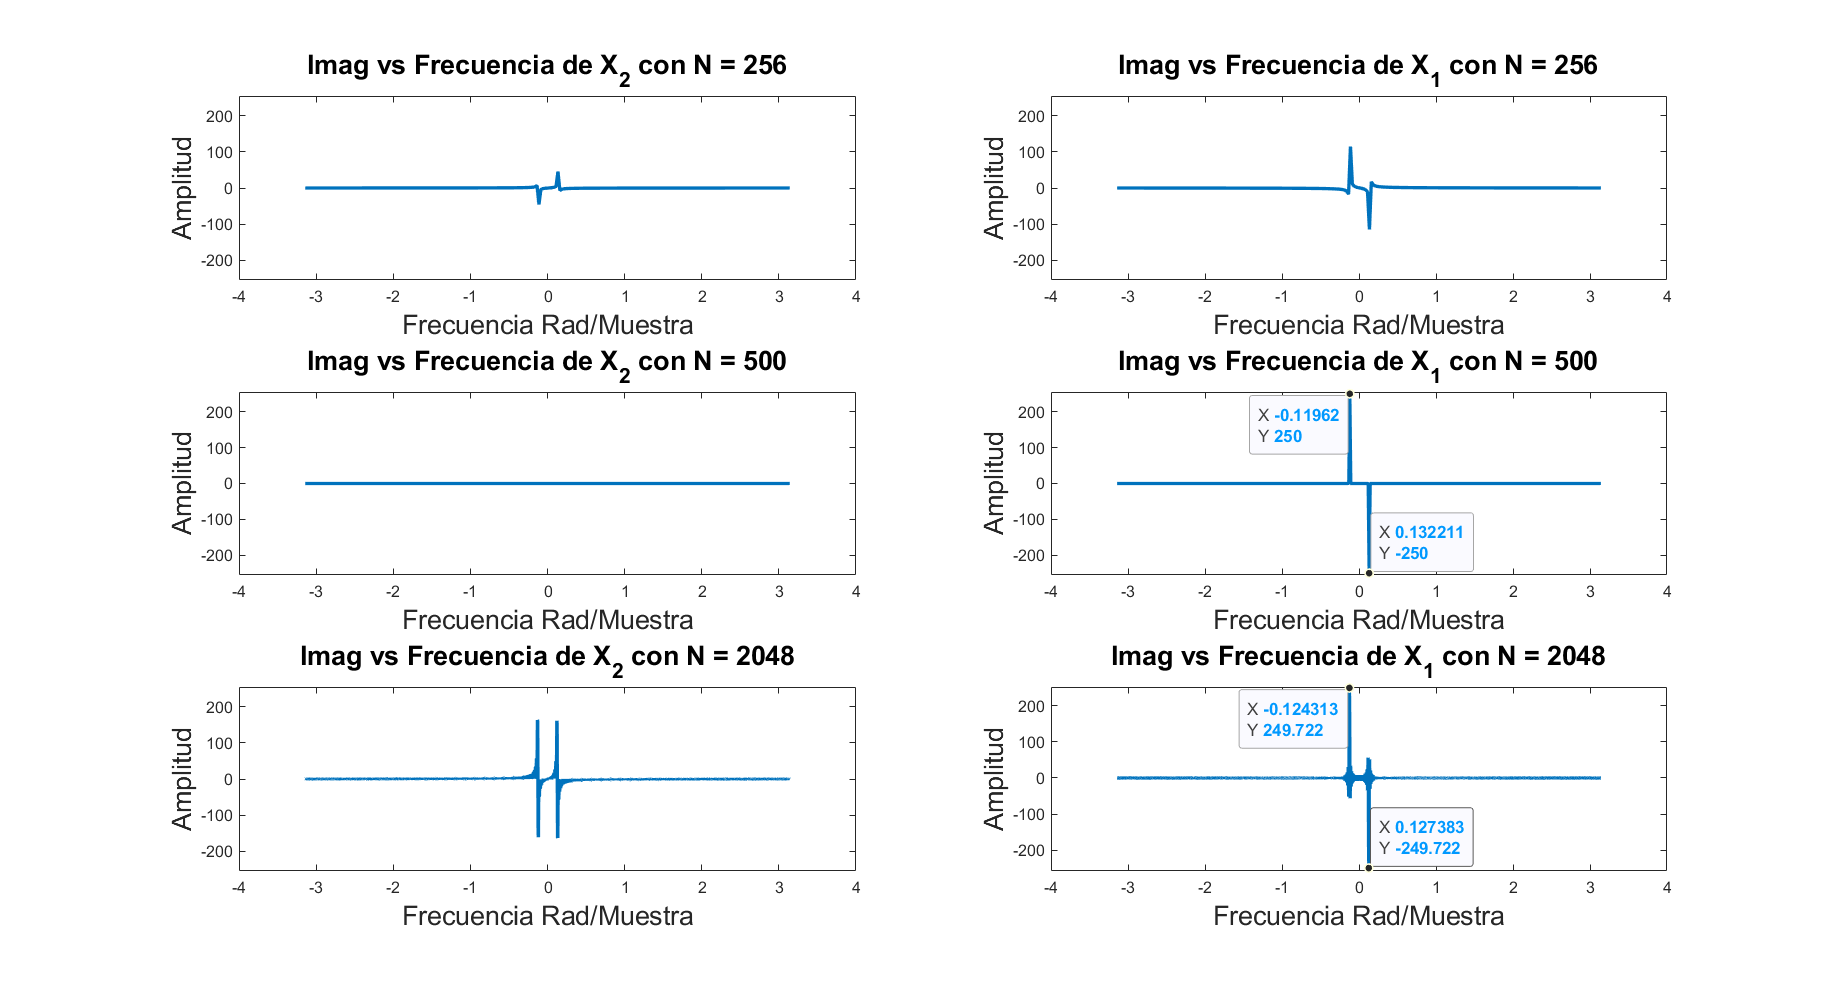
\includegraphics[width=1 \linewidth]{Figuras/I3)c.png}
\caption{Img vs Frecuencia para diferentes valores de N.}
\label{fig:I3)b}
\end{figure}

\begin{itemize}
    \item 
    Para $N=256$ se observa que la magnitud es inferior a los $250$ esperados y se acerca más a $128$, esto se debe a que solo se consideran las primeras $256$ muestras para el calculo de la DFT. Sin embargo la amplitud es menor a $128$ para ambas señales. Lo cual se debe a que $256$ no es una cantidad finita de períodos de la señal, por lo que al ser la DFT períodica, se genera una distorsión en el ''corte'' entre períodos. Esto también provoca que la DFT tenga tanto parte real como imaginaria en los dos casos.
    \item
    Para $N=500$ se observa que, tal como es de esperarse, la magnitud es de $250$, $X1$ tiene solo parte real y $X2$ tiene solo parte imaginaria. Generando las DFT esperadas para un coseno y un seno respectivamente. Esto se debe a que 500 muestras es un número completo de períodos de estas señales.
    \item
    Para $N=2048$, al tomar más muestras que las contenidas en la señal, la DFT rellena con ceros las muestras faltantes, generando distorsión en la amplitud y fase de la señal. Se observa que la amplitud es cercana a los $250$ esperados pero cada peak está rodeado de una sinc por el enventanamiento cuadrado.
\end{itemize}

\end{enumerate}
\end{enumerate}
%  ^^^^^^^^^^^^^^^^ mucho de esta wea no tengo idea q es, aidua. ^^^^^^^^^^^^^^^^^^^^
%  ||||||||||||||||                                              |||||||||||||||||||| 
%%%%%%%%%%%%%%%%%%%%%%%%%%%%%%%%%%%%%%%%%%%%%%%%%%%%%%%%%%%%%%%%%%%%%%%%%%%%%%%%%
%
%-------------II. ESTIMACI ́ON DEFRECUENCIA ENPRESENCIA DERUIDOS----------------------------%
%
%%%%%%%%%%%%%%%%%%%%%%%%%%%%%%%%%%%%%%%%%%%%%%%%%%%%%%%%%%%%%%%%%%%%%%%%%%%%%%%%%
\section{Estimación de frecuencias en presencia de ruidos}
Se genera la siguiente señal:
\begin{equation}
    s_1 = \frac{1}{2} cos(2 \pi 100 t)+1.5 cos(2 \pi 500 t)
\end{equation}
A la cual se le suma el ruido de la siguiente manera:
\begin{lstlisting}
fs = 5000;
t=0:1/fs:0.1-1/fs;
s_1 = 0.5*cos(2*pi*100*t)+1.5*cos(2*pi*500*t);
senal = s_1+(sqrt(2)*randn(1,500));
\end{lstlisting}
\begin{itemize}
\item El gráfico de la señal en el tiempo se muestra en la Figura \ref{IIa}, donde no se distingue $s_1$, ni sus frecuencias debido al ruido.

\begin{figure}[H]
\centering
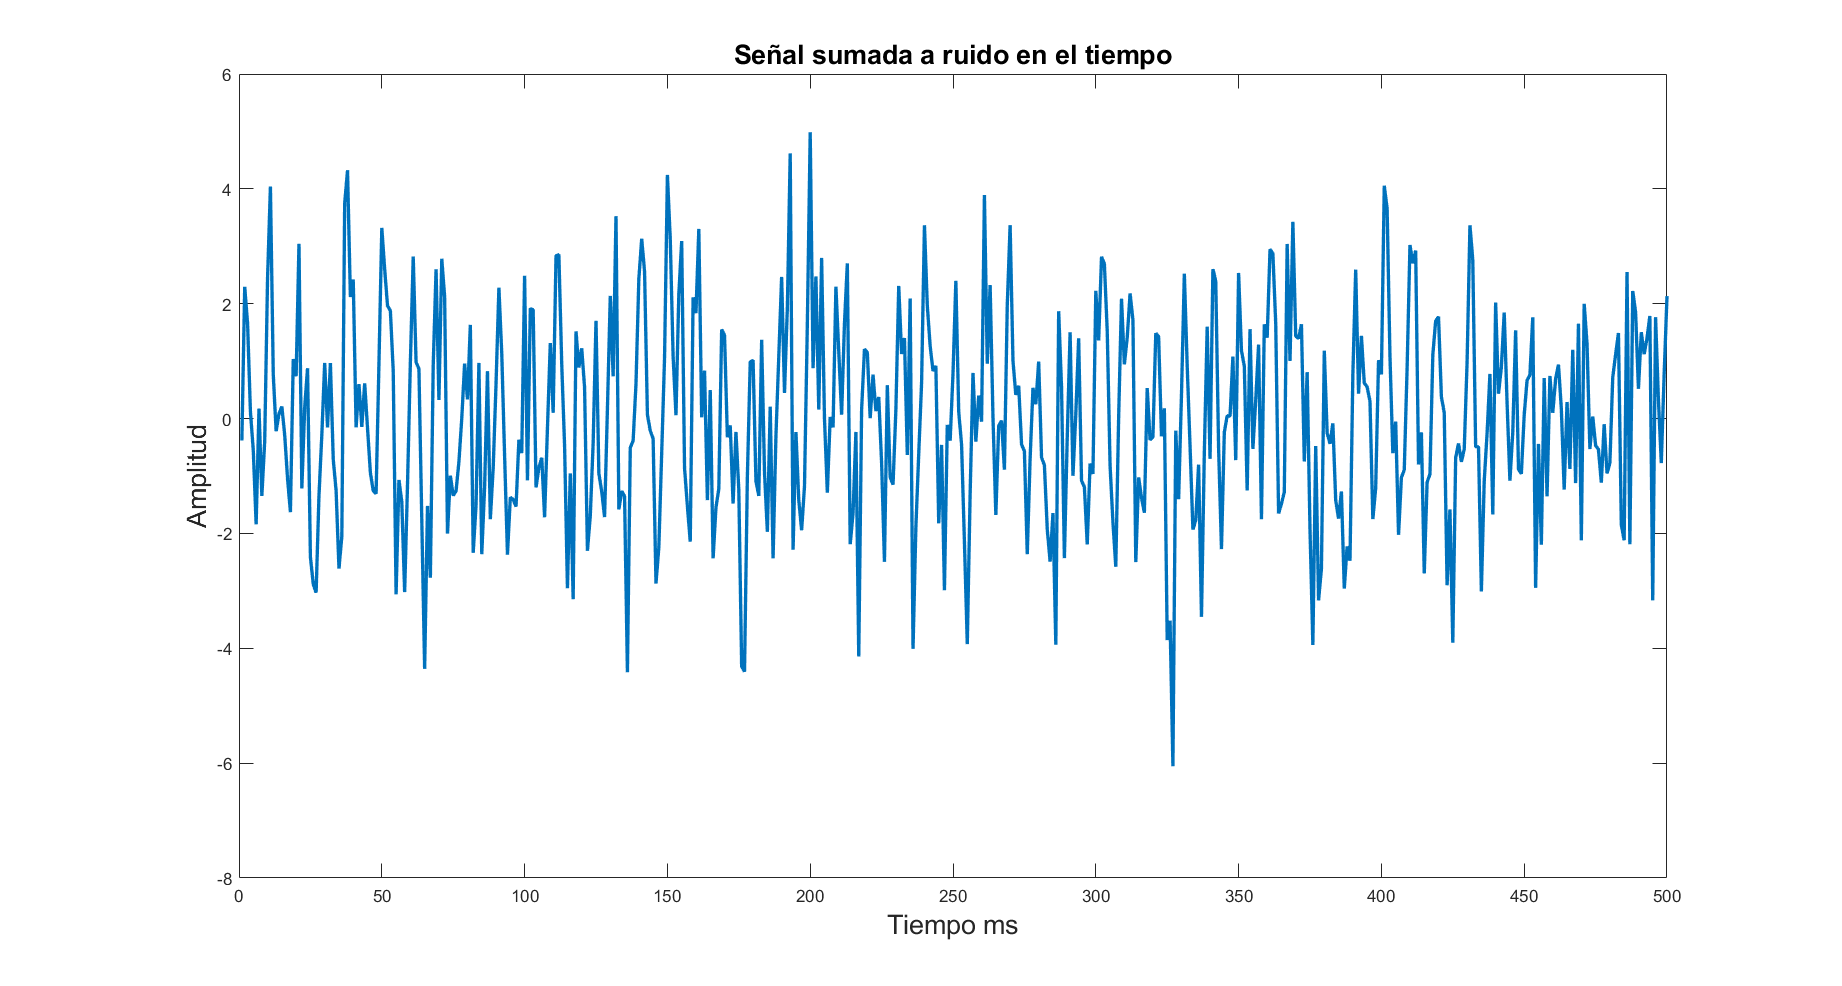
\includegraphics[width=1 \linewidth]{Figuras/IIa.png}
\caption{Señal $s_1$ más ruido comparación en magnitud.}
\label{IIa}
\end{figure}



\item El gráfico de la magnitud del espectro de la señal con y sin ruido se muestra en la Figura \ref{IIb}, donde se distinguen claramente las frecuencias de interés a pesar del ruido de la señal. Se destaca que las amplitudes que acompañan a cada una de las frecuencias de interés, también corresponden a las esperadas, siendo estas la cantidad de muestras sobre dos, multiplicado por la amplitud de cada uno de los armónicos.

\begin{figure}[H]
\centering
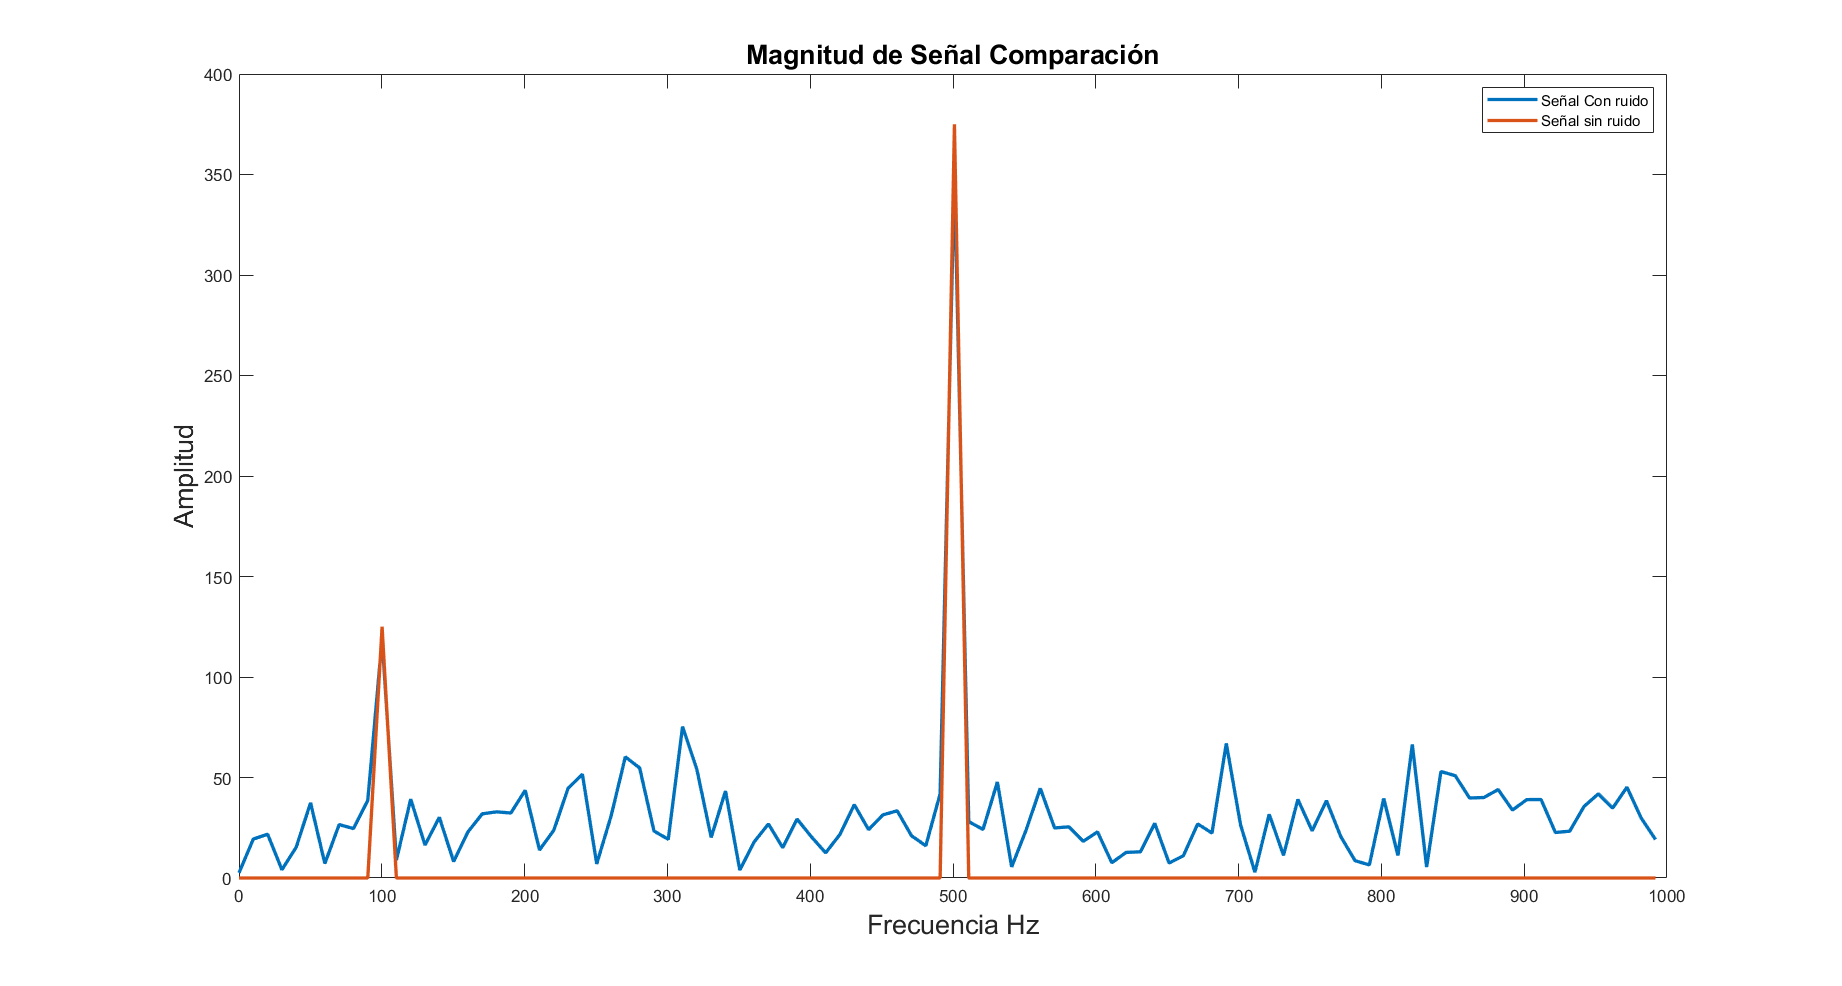
\includegraphics[width=1 \linewidth]{Figuras/IIb.png}
\caption{Señal $s_1$ más ruido en el tiempo.}
\label{IIb}
\end{figure}

\item El gráfico de la magnitud del espectro en decibeles con y sin ruido se muestra en la Figura \ref{IIc}, donde vemos que aproximadamente hay 28 decibeles desde la señal con mayor amplitud hasta la capa de ruido.

\begin{figure}[H]
\centering
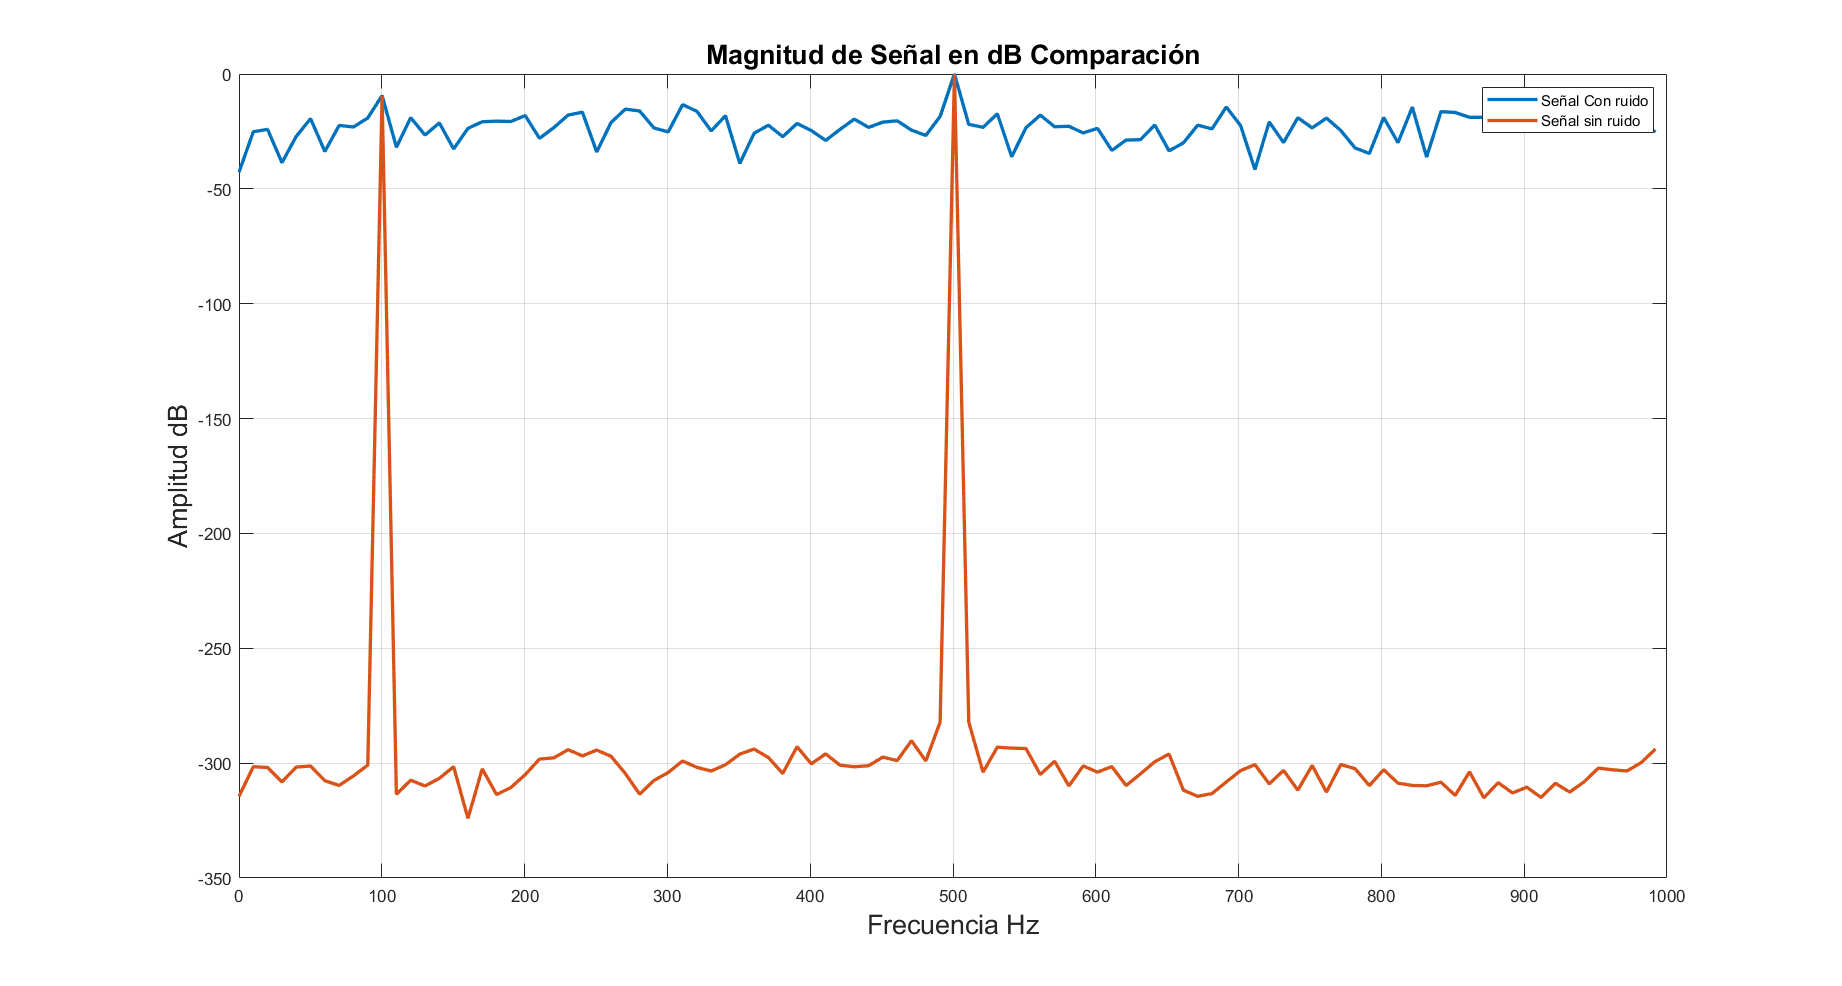
\includegraphics[width=1 \linewidth]{Figuras/IIc.png}
\caption{Señal $s_1$ más ruido, comparación en decibeles.}
\label{IIc}
\end{figure}

Al aumentar la duración de la señal a 1 segundo, se consigue el resultado en mostrado en la Figura \ref{IId}, donde la señal de más duración tiene una resolución mucho mayor en su espectro en frecuencia, esto se debe a que, al contar con más muestras en el tiempo, se tienen del mismo modo más muestras en el espectro de frecuencia.

Se observa que la diferencia en amplitud entre la señal y el ruido aumenta al aumentar la duración de la señal. Esto se debe a que la amplitud de los peaks de la señal dependen directamente del número de muestras, sin embargo el ruido es uniforme en el espectro, por lo que su magnitud es invariante al aumentar el largo.
% ayuda, no recuerdo muy bien; se debe a que por al aumentar la duración de la señal, esta tiene más muestras que suman, lo q aumenta la magnitud en las frecuencias de interes, alejando estas del piso de ruido? o taria bien hablar de resolución tmb?

\begin{figure}[H]
\centering
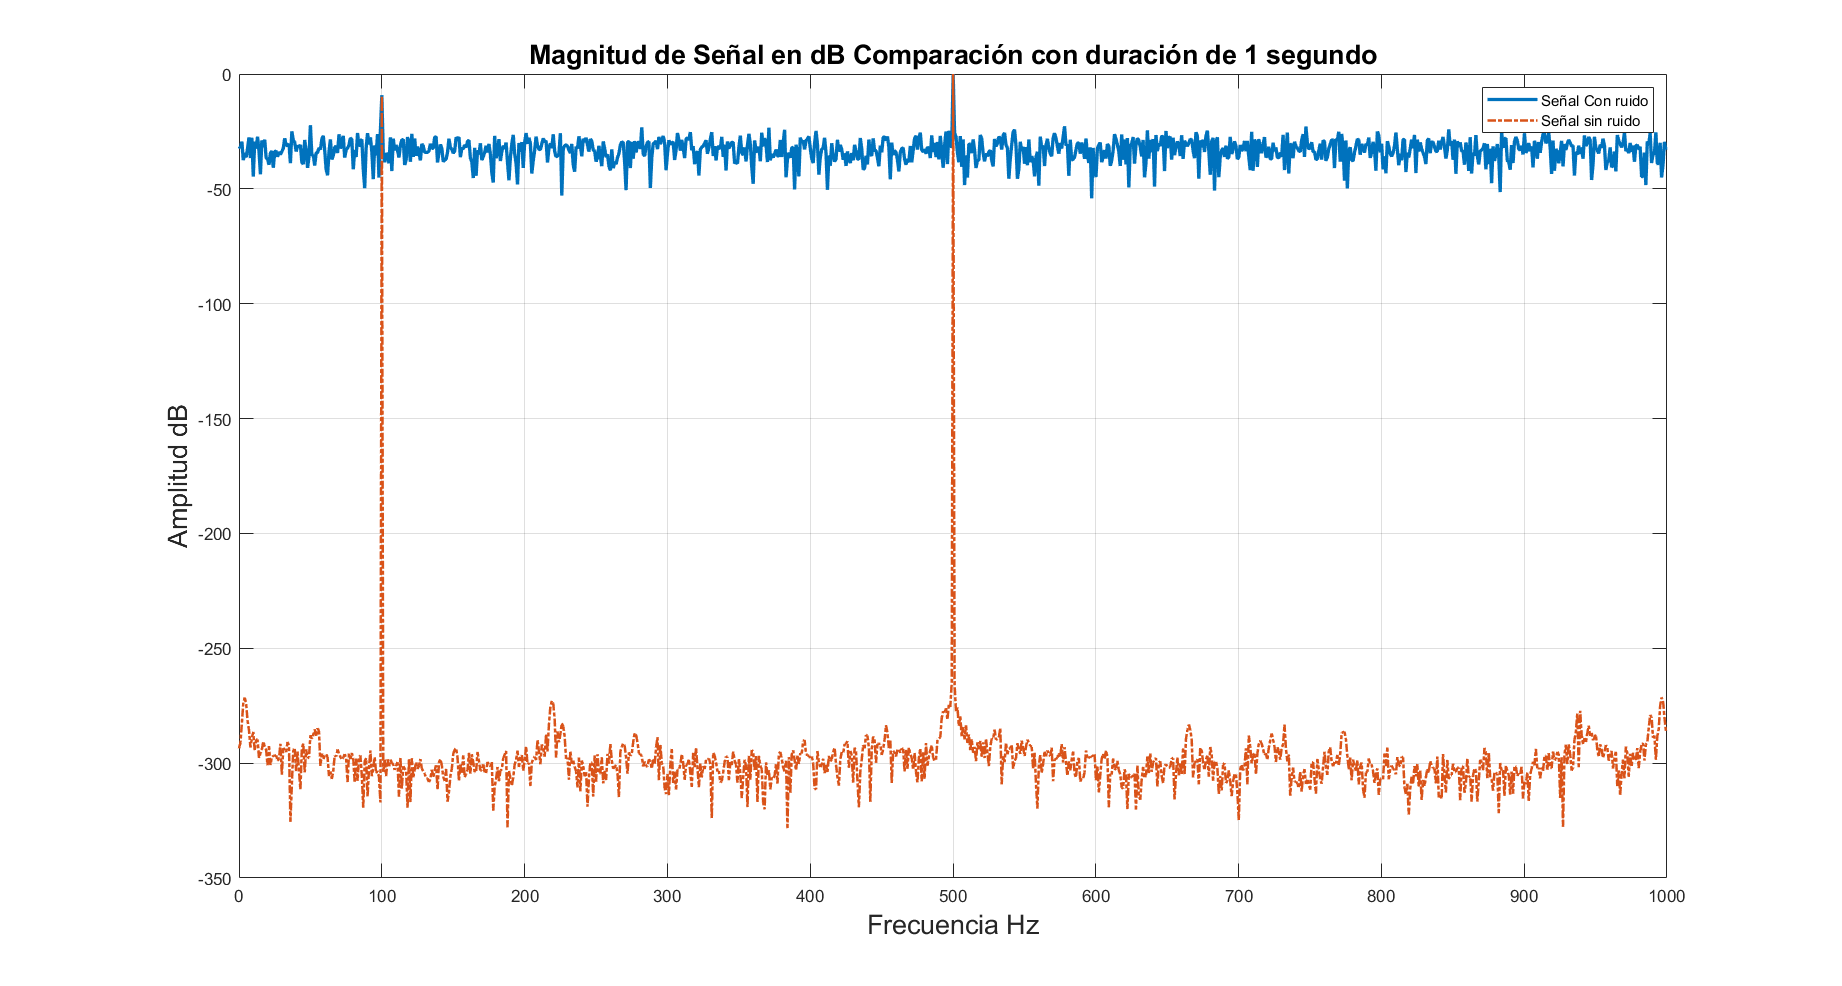
\includegraphics[width=1 \linewidth]{Figuras/IId.png}
\caption{Señal $s_1$ más ruido, comparación en decibeles, duración 1 s.}
\label{IId}
\end{figure} 

\end{itemize}
%%%%%%%%%%%%%%%%%%%%%%%%%%%%%%%%%%%%%%%%%%%%%%%%%%%%%%%%%%%%%%%%%%%%%%%%%%%%%%%%%
%
%---------III. FILTRADO DESE ̃NALES EN ELDOMINIO DE LAFRECUENCIAB--------------------%
%
%%%%%%%%%%%%%%%%%%%%%%%%%%%%%%%%%%%%%%%%%%%%%%%%%%%%%%%%%%%%%%%%%%%%%%%%%%%%%%%%%
\section{Filtrado de señales en el dominio de la frecuencia}

Se aplica $fft$ a la señal $nspeech$ original, obteniendo su espectro en frecuencia, el cual se muestra con una amplitud en dB en la Figura \ref{IIIa}, donde se extrae la frecuencia del tono no deseado, igual a $f = 1685.4 ~ Hz$.

\begin{figure}[H]
\centering
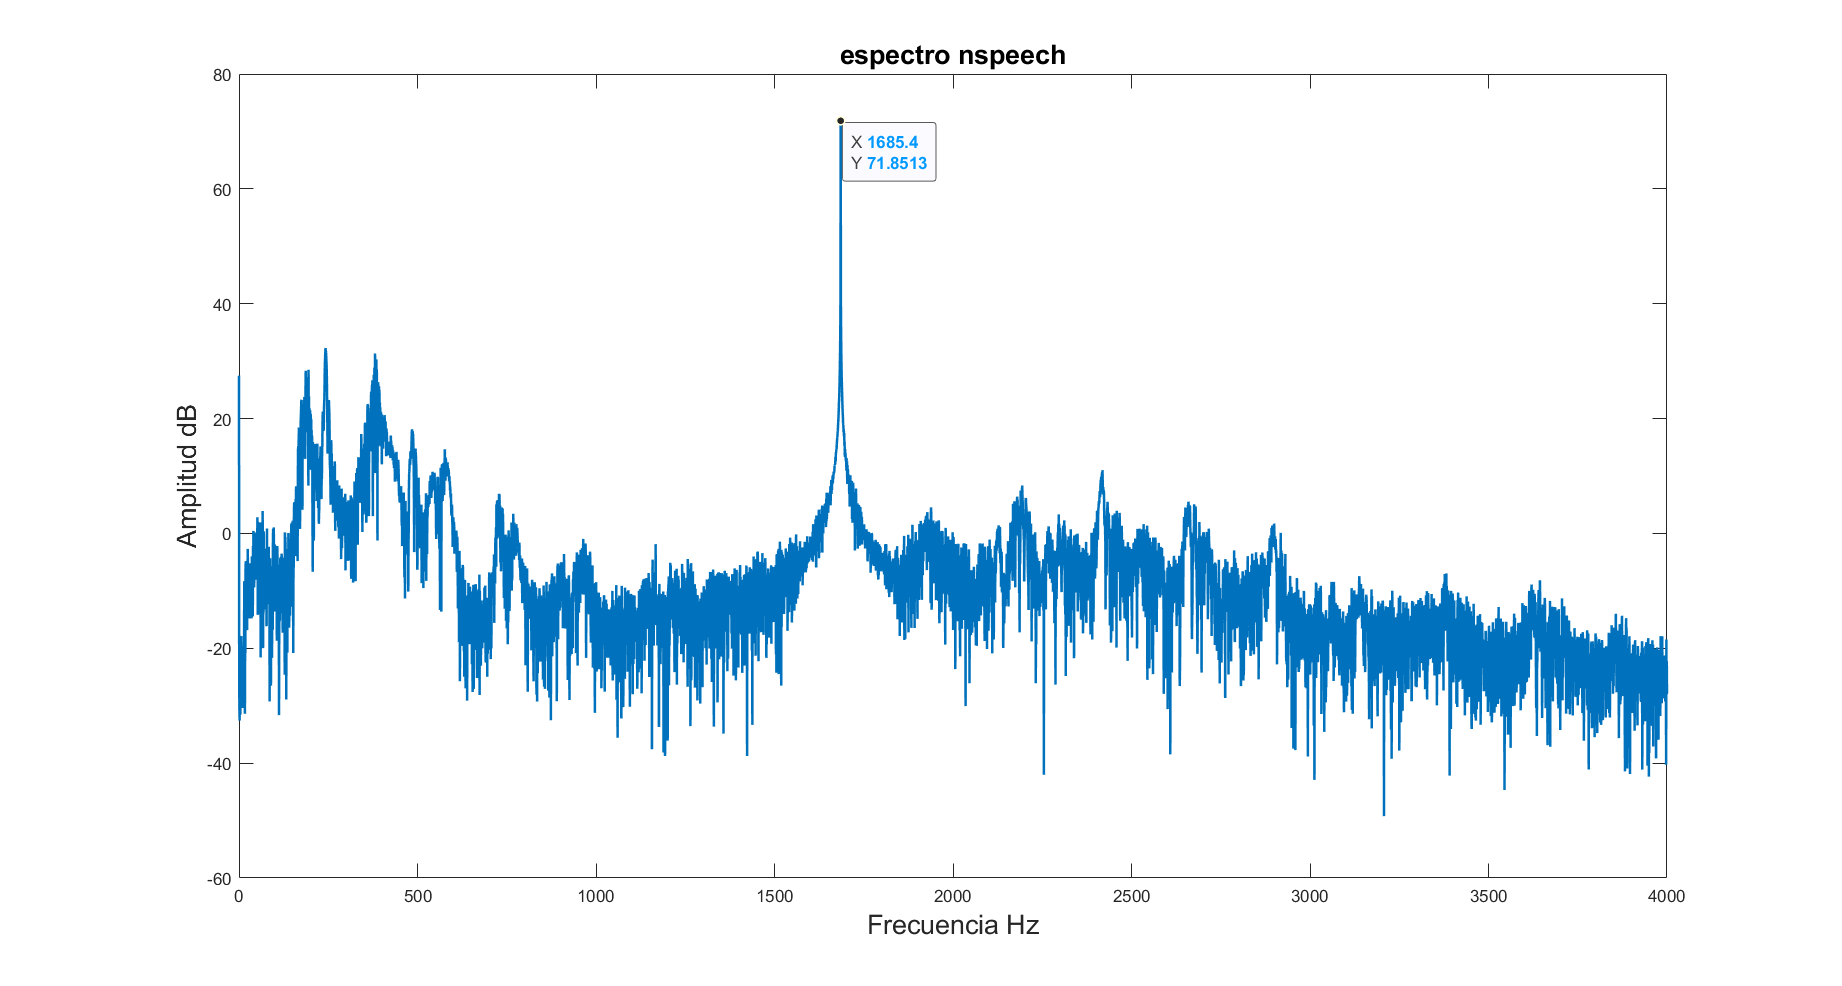
\includegraphics[width=1 \linewidth]{Figuras/IIIa.png}
\caption{Magnitud del espectro de $nspeech$ en dB.}
\label{IIIa}
\end{figure} 

Se Obtiene el parámetro $\theta = 2 \pi \frac{f}{f_s}$, por lo que $\theta = 1.3237 ~ Rad/Muestra$. \\

Se muestra la magnitud en dB del filtro en la Figura \ref{IIIb} donde se aplico el valor de $\theta$. En la gráfica se observa una caída de cerca de 70 dB en la frecuencia de interés.

\begin{figure}[H]
\centering
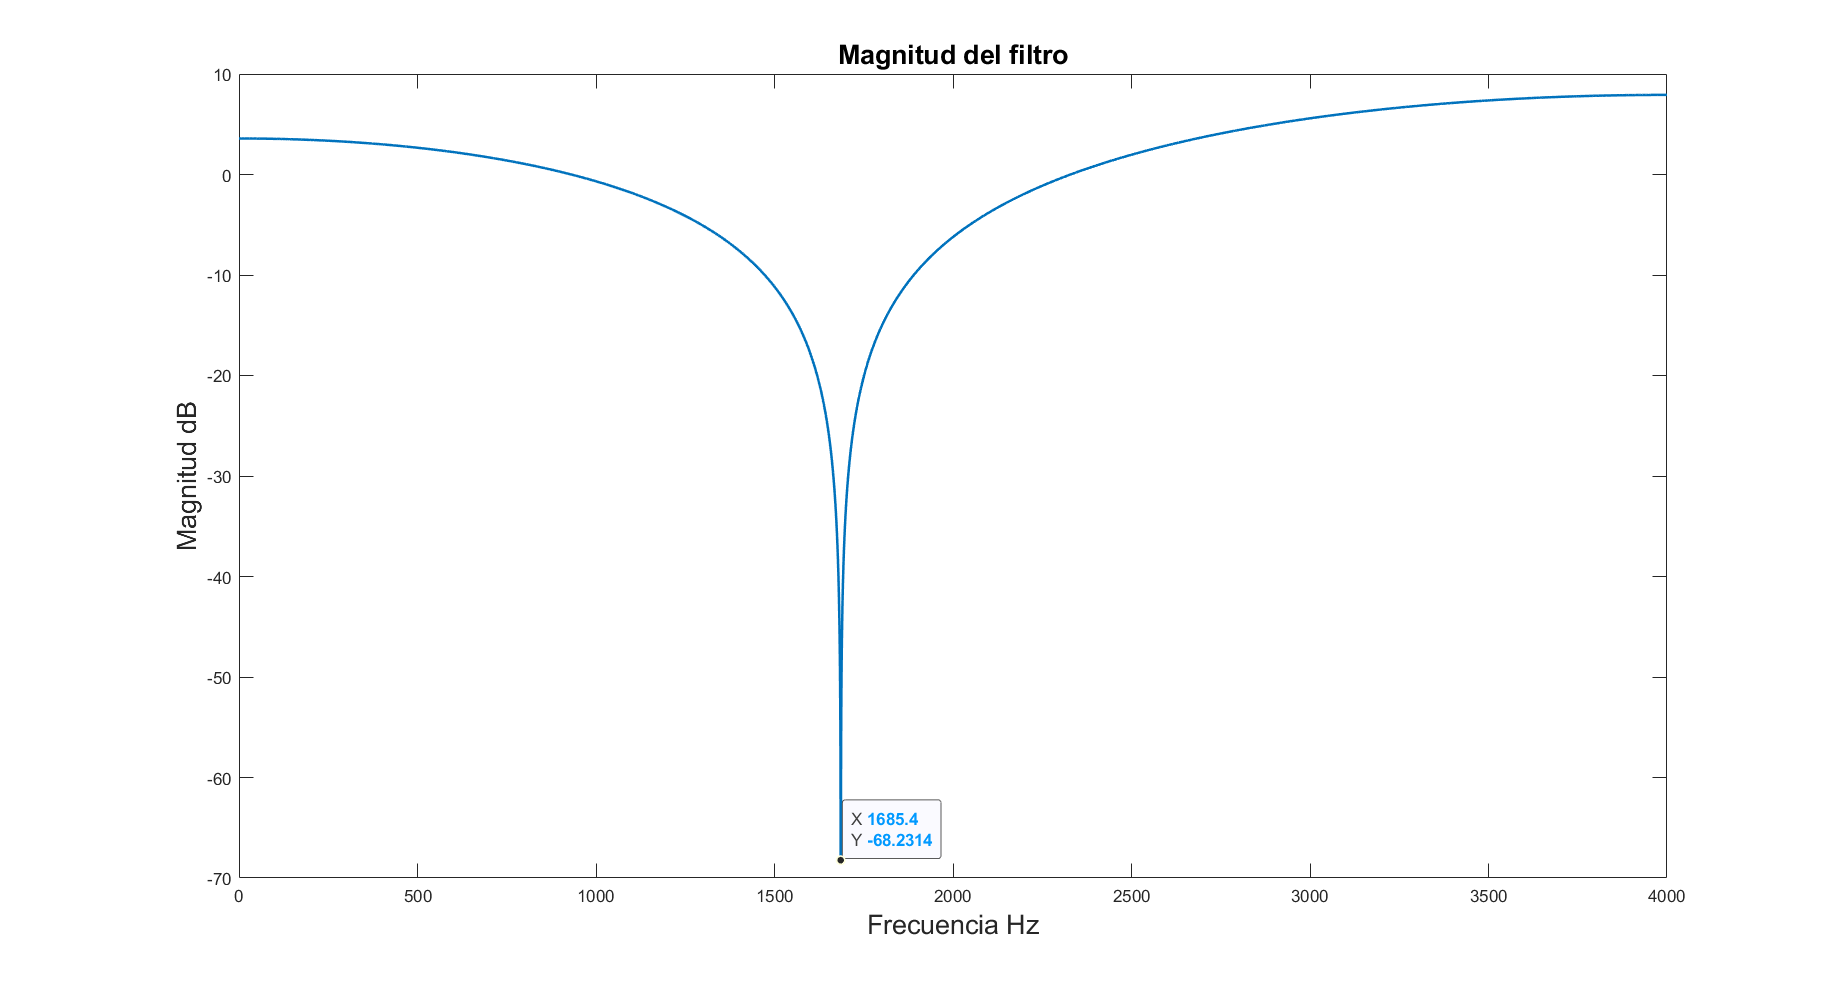
\includegraphics[width=1 \linewidth]{Figuras/IIIb.png}
\caption{Magnitud del filtro en dB.}
\label{IIIb}
\end{figure} 

Se aplica el filtrado a la $DFT$ de la señal $nspeech$ mediante una operación punto a punto segun el siguente codigo de $Matlab$:
\begin{lstlisting}
f=1685.4; 
w=2*pi*f/fs; %-> omega
filtro=1-2*cos(w)*exp(-j*2*pi*(w_vector)/fs)+exp(-2*j*2*pi*(w_vector)/fs);
fft_filtrada = fft_senal.*filtro;
\end{lstlisting}
El resultado de esta operación, con magnitud en dB, se muestra en la Figura \ref{IIIc}, donde se observa que el tono no deseado disminuye su amplitud cerca de 68 dB, que corresponde al rechazo del filtro. Si bien el tono no fue completamente eliminado, es prácticamente inaudible. 

\begin{figure}[H]
\centering
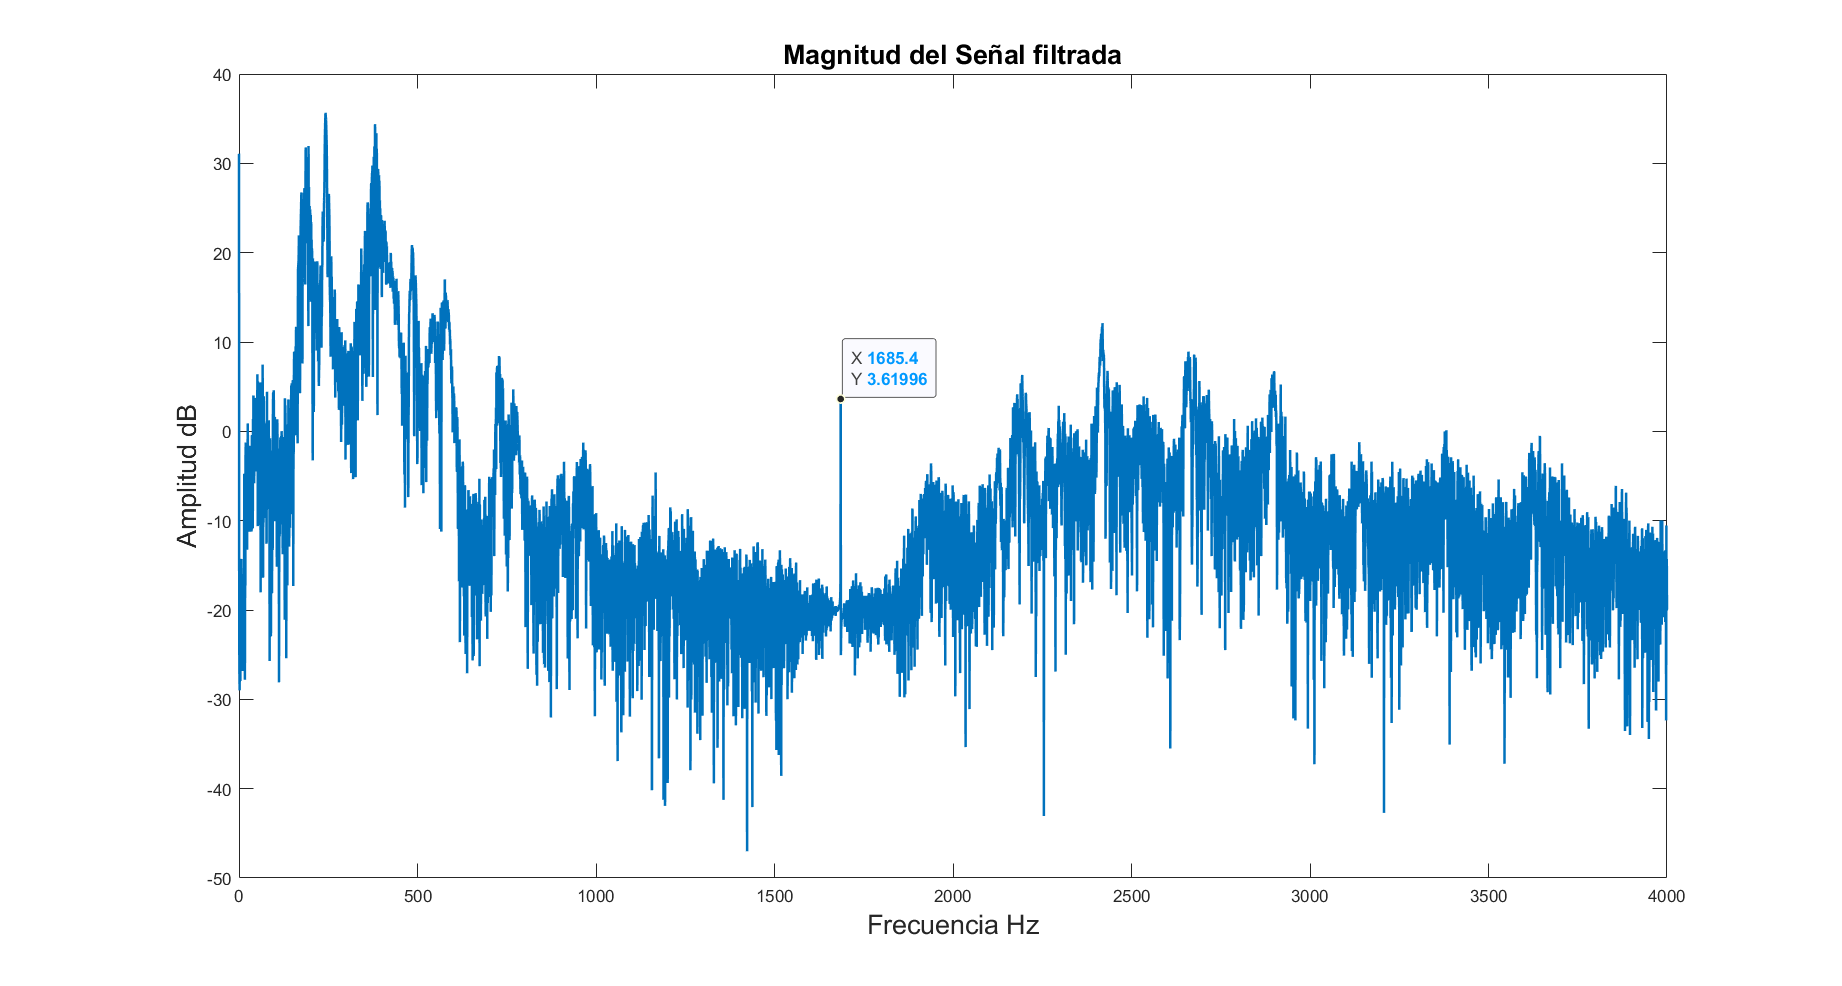
\includegraphics[width=1 \linewidth]{Figuras/IIIc.png}
\caption{Magnitud de la señal filtrada en dB.}
\label{IIIc}
\end{figure} 

El resultado de aplicar la transformada inversa $ifft$ se muestra en la Figura \ref{IIId}, Donde se observa la estructura temporal de la señal filtrada casi por completo recuperada comparada con la señal original que es prácticamente inteligible. al escuchar ambas señales, podemos entender completamente el mensaje de la señal filtrada a diferencia de la original, donde predomina el sonido del tono no deseado.\\

Tanto la señal original como la señal filtrada tienen el mismo numero de muestras. % no se a que se refiere con  ' que valor de N se requiere para reconstruir la señal completamente, ayuda 

\begin{figure}[H]
\centering
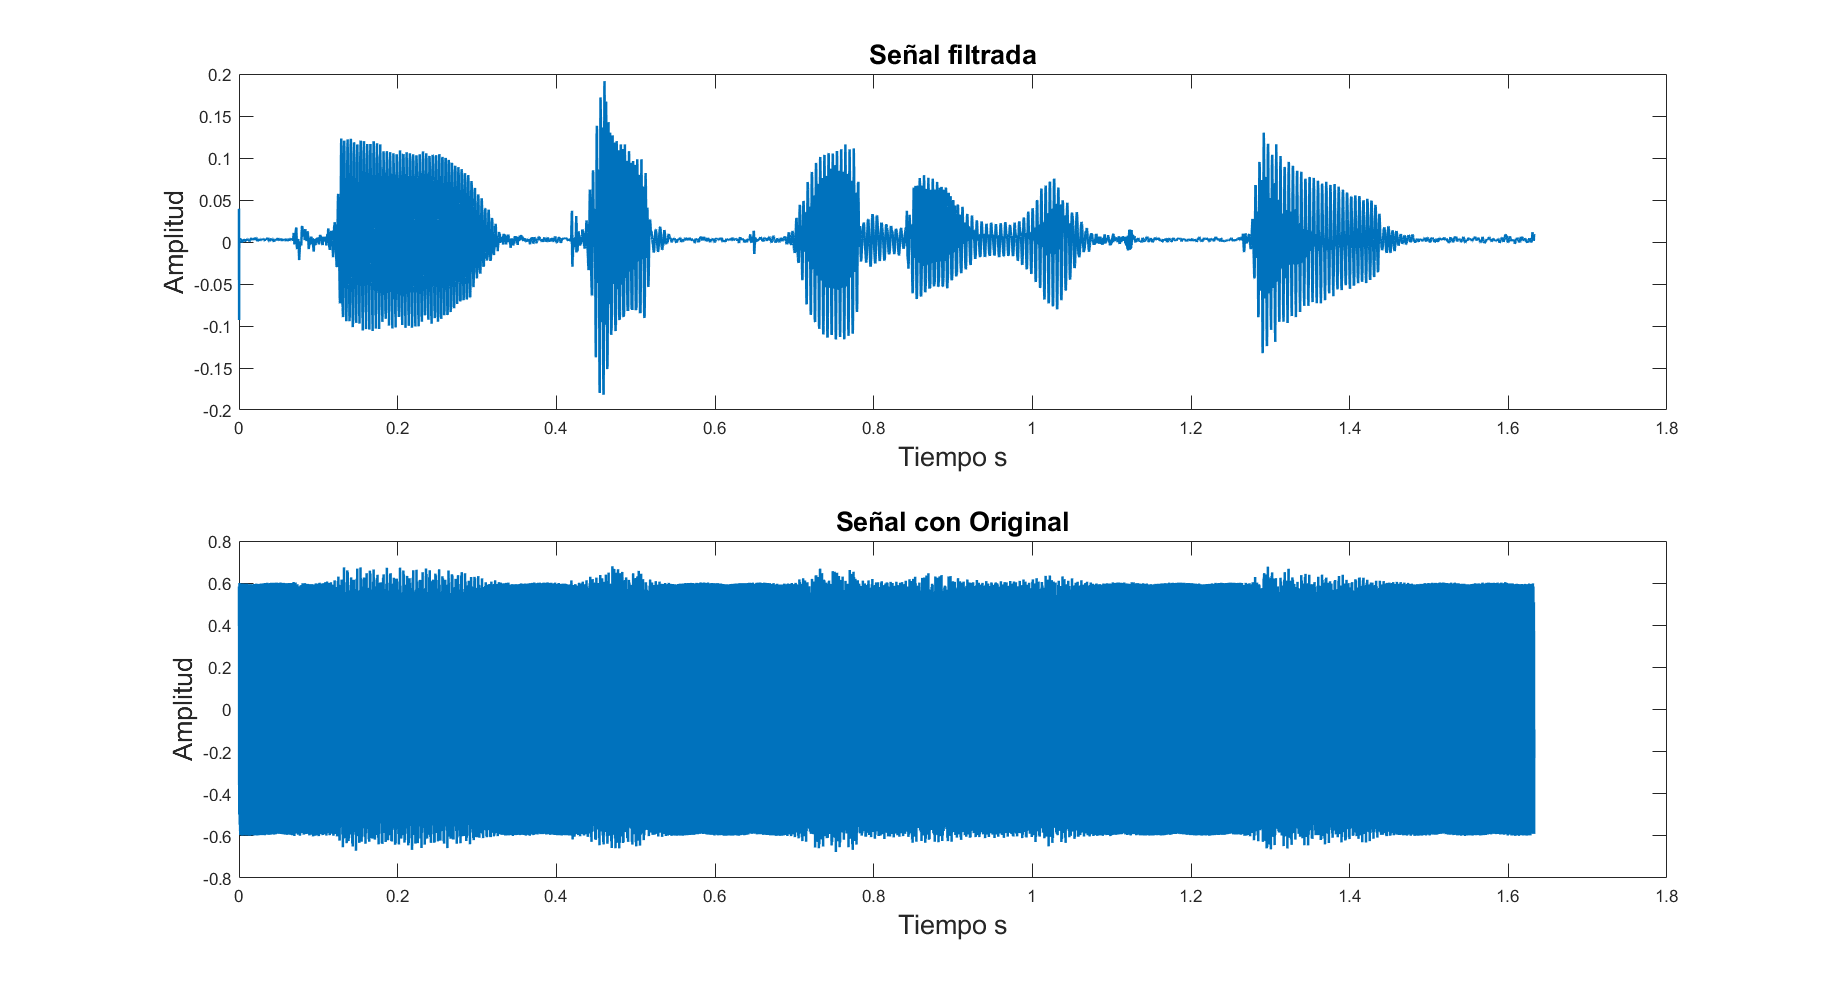
\includegraphics[width=1 \linewidth]{Figuras/IIId.png}
\caption{Señal filtrada vs Señal original en el tiempo.}
\label{IIId}
\end{figure} 

%%%%%%%%%%%%%%%%%%%%%%%%%%%%%%%%%%%%%%%%%%%%%%%%%%%%%%%%%%%%%%%%%%%%%%%%%%%%%%%%%
%
%---------C ́ALCULODIRECTO DE LADFT-----------------%
%
%%%%%%%%%%%%%%%%%%%%%%%%%%%%%%%%%%%%%%%%%%%%%%%%%%%%%%%%%%%%%%%%%%%%%%%%%%%%%%%%%
\section{Cálculo directo de la DFT}
La implementación en $MATLAB$ de la función $DFTsum$ se presenta a continuación:
\begin{lstlisting}
function X=DFTsum(x) 
N = length(x);
X = zeros([1,N]);
for k=1:length(x)
    for n=1:length(x)
        X(k)=X(k)+x(n)*exp(-j*2*pi*(k-1)*(n-1)/N);
    end
end
end
\end{lstlisting}
Donde se implementa la ecuación siguiente en forma directa utilizando dos ciclos for.
\begin{equation*}
    X^{(N)}[k] = \sum _{n = 0} ^{N-1} x[n] e ^{\frac{-j 2 \pi k n}{N}}
\end{equation*}
\begin{enumerate}[1)]
    \item%1)-------------------------------------------------------------------------%

Se prueba la función para $N = 8$ con las señal a continuación:
\begin{enumerate}
    \item $x_1[n] = \delta [n]$ 
    \item $x_2[n] = 1$
    \item $x_3[n] = e^{\frac {-j 2 \pi n}{N}}$
    \item $x_4[n] = cos( \frac{2 \pi n}{N})$
\end{enumerate}
El resultado de probar estas señales con el filtro diseñado y la función $fft$ de $MATLAB$ se muestra en la Figura \ref{IV1}, que son equivalentes en magnitud.

\begin{figure}[H]
\centering
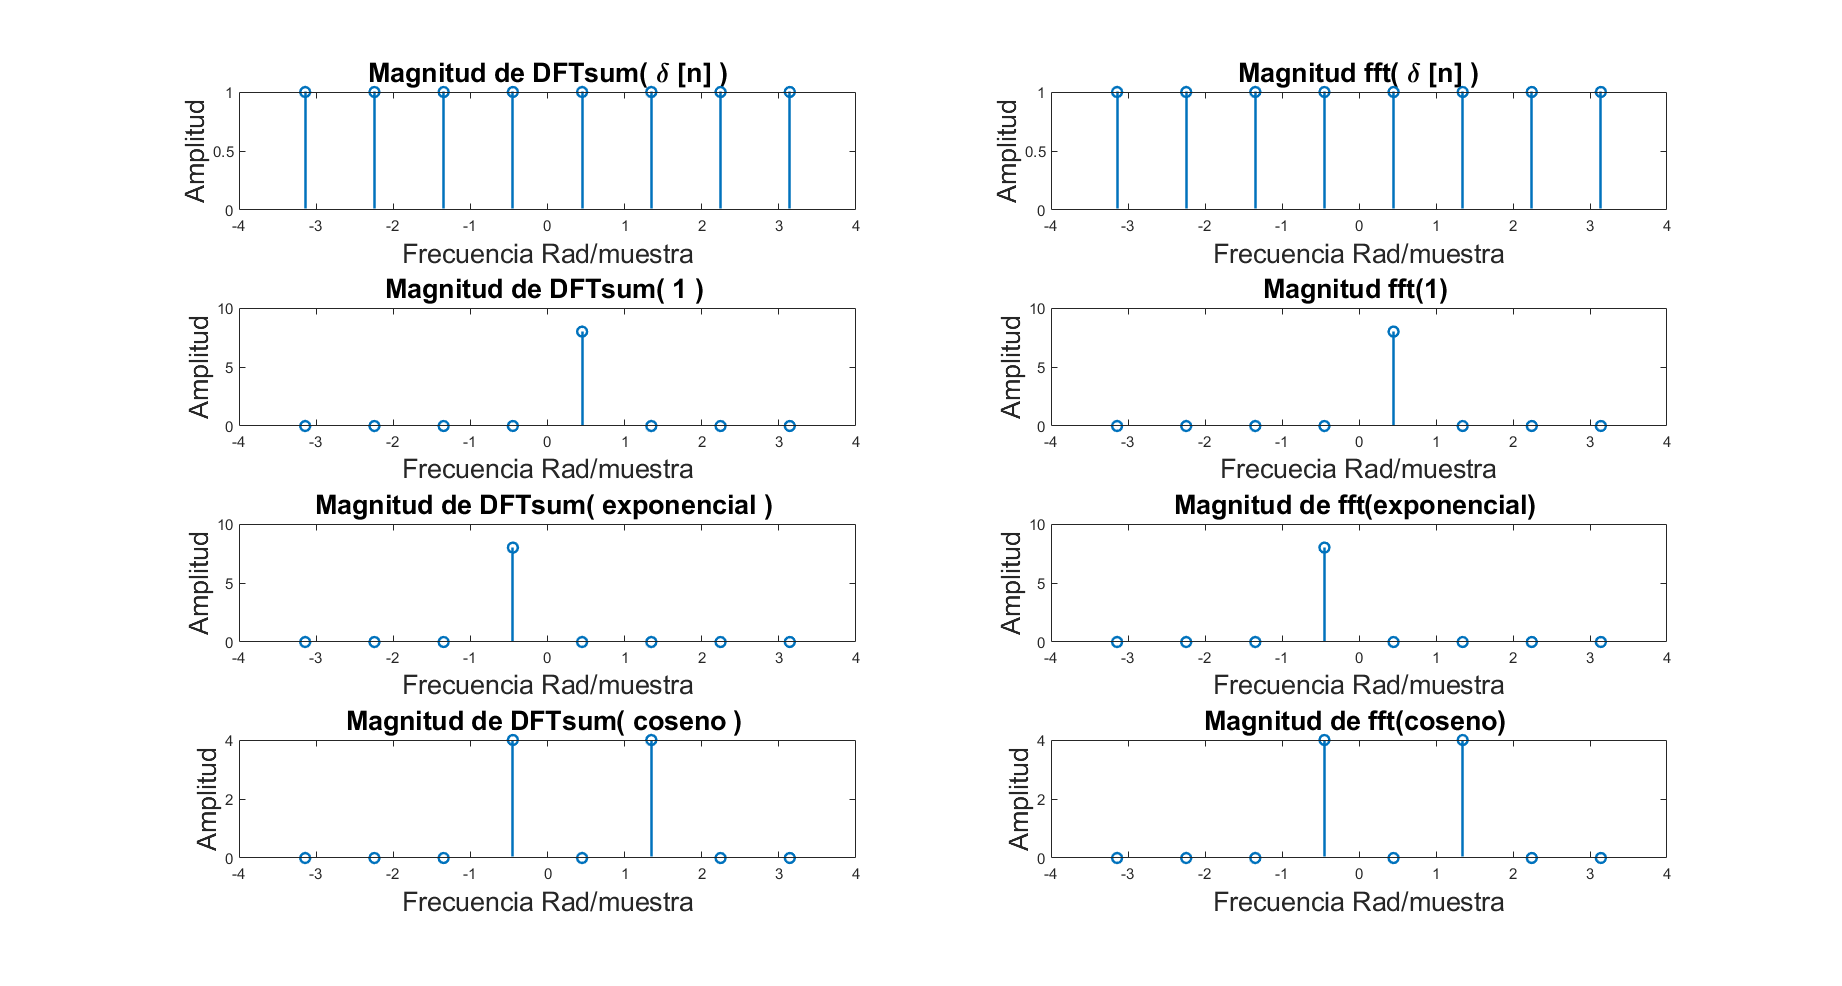
\includegraphics[width=1 \linewidth]{Figuras/IV1.png}
\caption{Comparación con las distintas funciones.}
\label{IV1}
\end{figure}

El error cuadrático medio el resultado proporcionado por las funciones $DFTsum$ y $fft$ se muestra para cada señal en la tabla \ref{tab:1}, Donde el error mostrado es pequeño y se aprecia que los resultados obtenidos son aceptables.

\begin{table}[H]
        \centering
        \begin{tabular}{|c|c|c|}
        \hline
            Señal     & MSE \\ \hline
            $x_1[n]$ & 0 \\
            $x_2[n]$ & 3.8323e-30 \\
            $x_3[n]$ & 9.8353e-30 \\
            $x_4[n]$ & 3.1977e-30 \\\hline
        \end{tabular}
        \caption{MSE entre Función $DFTsum$ y $fft$ de $MATLAB$}
        \label{tab:1}
\end{table}

    
    \item %2)-------------------------------------------------------------------------%
       
El calculo de la DTFT de las señales se muestra a continuación:
\begin{enumerate}
    \item
\begin{equation*}
\begin{split}
    x_1 [n] &\xleftrightarrow{\text{DTFT}} \sum _{ n = 0} ^{7} \delta [n] e^{-j \omega n} \\
    x_1 [n] &\xleftrightarrow{\text{DTFT}} 1 
\end{split}
\end{equation*}

    \item 
\begin{equation*}
\begin{split}
    x_2 [n] &\xleftrightarrow{\text{DTFT}} \sum _{ n = 0} ^{7} 1 e^{-j \omega n} \\
    x_2 [n] &\xleftrightarrow{\text{DTFT}} e^{-j \omega 7/2}\frac{sin(4\omega )}{sin(\omega/2)} \\
\end{split}
\end{equation*}

    \item Sea $\omega _0 = \frac{ 2 \pi }{N}$ 
\begin{equation*}
\begin{split}
    x_3 [n] &\xleftrightarrow{\text{DTFT}} \sum _{ n = - \infty} ^{\infty} e^{-j \omega _0 n} e^{-j \omega n} \\
    x_3 [n] &\xleftrightarrow{\text{DTFT}} 2 \pi \delta ( \omega - \omega _0 )\ast e^{-j \omega 7/2}\frac{sin(4\omega )}{sin(\omega/2)} , ~~~~ \omega \in [0 , 2 \pi)  \\
    x_3[n]&\xleftrightarrow{\text{DTFT}} 2 \pi e^{-j (\omega-\omega_0) 7/2}\frac{sin(4(\omega-\omega_0) )}{sin((\omega-\omega_0)/2)} \\
\end{split}
\end{equation*}

    \item Sea $\omega _0 = \frac{ 2 \pi }{N}$ 
\begin{equation*}
\begin{split}
    x_4 [n] &\xleftrightarrow{\text{DTFT}} \sum _{ n = - \infty} ^{\infty} cos( \omega _0 n) e^{-j \omega n} \\
    x_4 [n] &\xleftrightarrow{\text{DTFT}} \pi( \delta ( \omega + \omega _0 ) +  \delta ( \omega - \omega _0 ))\ast e^{-j \omega 7/2}\frac{sin(4\omega )}{sin(\omega/2)} ,~~~~ \omega \in [0 , 2 \pi) \\
     x_3[n]&\xleftrightarrow{\text{DTFT}} \pi e^{-j (\omega-\omega_0) 7/2}\left(\frac{sin(4(\omega-\omega_0) )}{sin((\omega-\omega_0)/2)} + \frac{sin(4(\omega+\omega_0) )}{sin((\omega+\omega_0)/2)} \right) \\
\end{split}
\end{equation*}
\end{enumerate}
    \item %3)-------------------------------------------------------------------------%
Se comparan las señales generadas por la función $DTFsum$ y $fft$ con el siguiente script de $MATLAB$
\begin{lstlisting}
fs=5000;
t=0:1/fs:1-1/fs;
x1=cos(2*pi*100*t);
dft_cos=DFTsum(x1(1:500));
fft_cos=fft(x1(1:500));
error_plot = (abs(dft_cos)-abs(fft_cos)).^2
MSE=immse(dft_cos,fft_cos)
\end{lstlisting}
Con lo que obtenemos un $MSE$ de 1.9344e-24, y se obtiene el gráfico mostrado en la Figura \ref{IV3}, donde se aprecia como el error aumenta al aumentar la frecuencia, pero sigue siendo un error despreciable.

\begin{figure}[H]
\centering
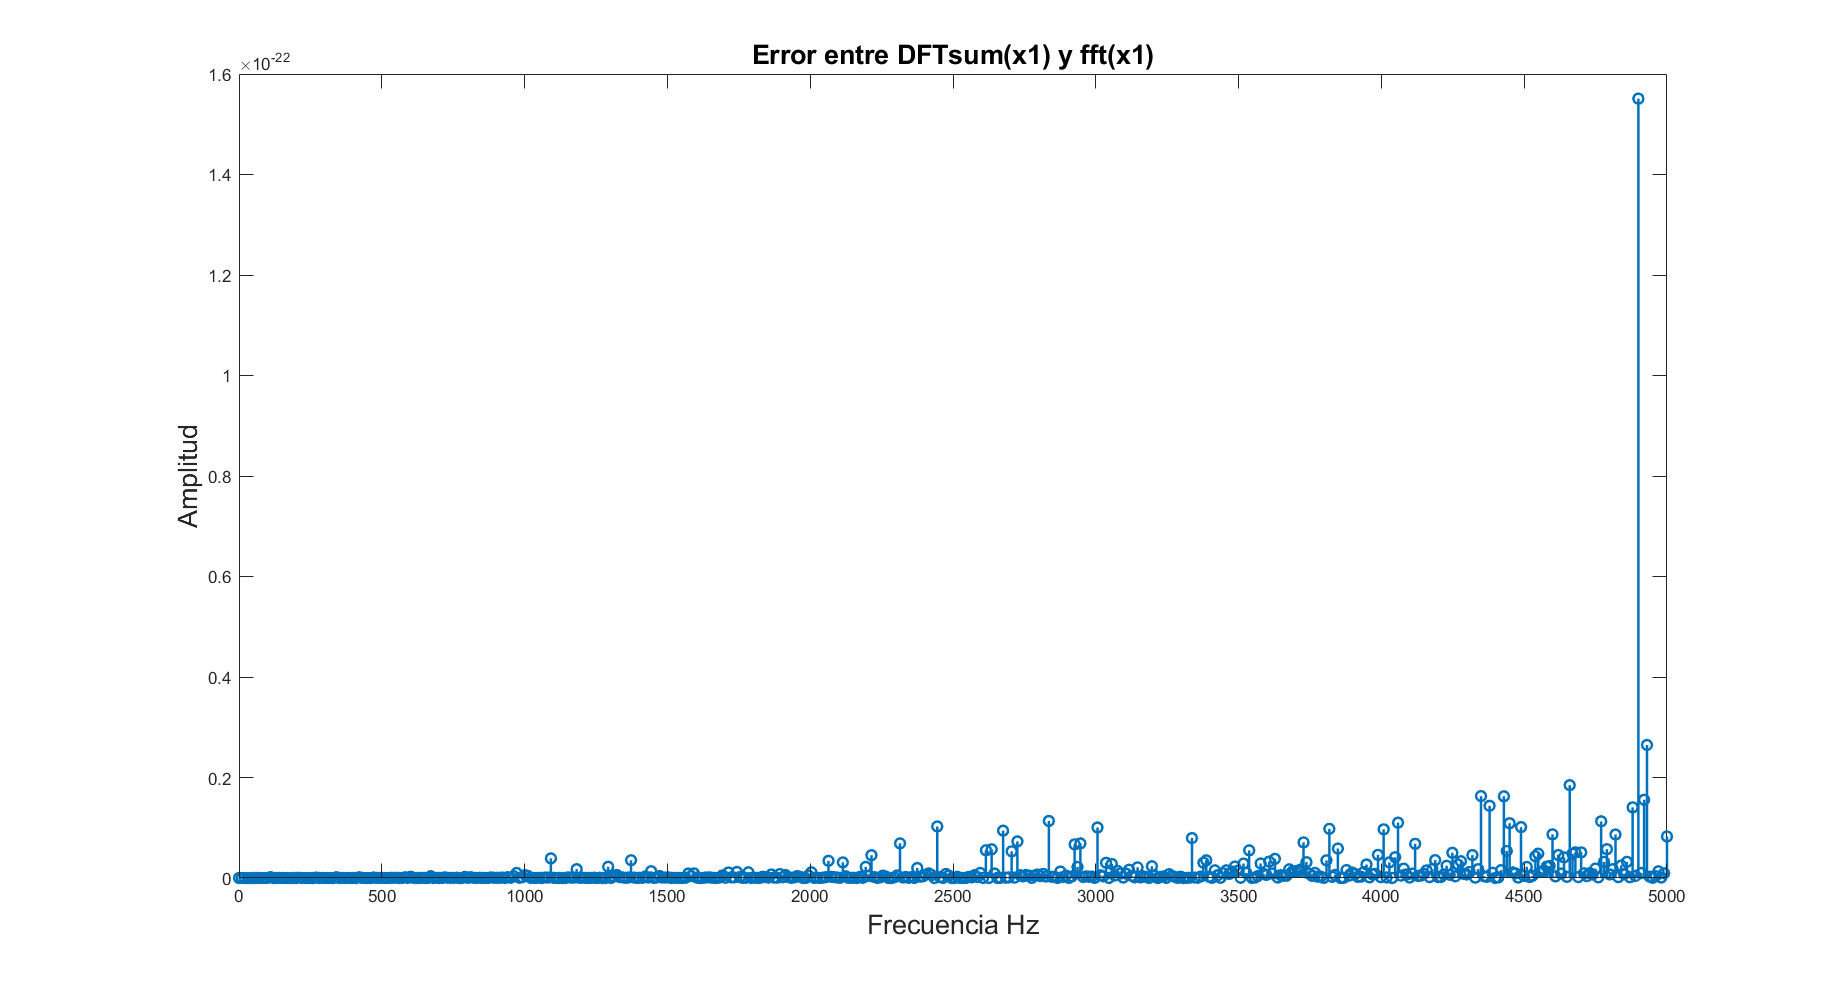
\includegraphics[width=1 \linewidth]{Figuras/IV3.png}
\caption{Magnitud del error entre usar DFTsum y fft.}
\label{IV3}
\end{figure}

\end{enumerate}
%%%%%%%%%%%%%%%%%%%%%%%%%%%%%%%%%%%%%%%%%%%%%%%%%%%%%%%%%%%%%%%%%%%%%%%%%%%%%%%%%
%
%--V. Calculo Matricial de la DFT------------------------%
%
%%%%%%%%%%%%%%%%%%%%%%%%%%%%%%%%%%%%%%%%%%%%%%%%%%%%%%%%%%%%%%%%%%%%%%%%%%%%%%%%%
\section{Cálculo matricial de la DFT}
\begin{enumerate}[1)]
    \item %1)--------------------------------------------------------------------------

La implementación en $MATLABde$ la función $genAmatrix$ se presenta a continuación:
\begin{lstlisting}
function A=genAmatrix(N)
A = zeros([N,N]);
for k=1:N
    for n=1:N
    A(k,n)=exp(-2*j*pi*(k-1)*(n-1)/N);
    end
end
end
\end{lstlisting}
A continuación se muestra la implementación de $DFTmatrix$:
\begin{lstlisting}
function X=DFTmatrix(x)
N = length(x);
X = zeros([1,N]);
A = genAmatrix(N);
X = x*A;
end
\end{lstlisting}
En la tabla \ref{tab:2} se muestra el error entre la función creada y la proporcionada por $MATLAB$, donde, al duplicar N el error aumenta en un orden de magnitud. Estos errores siguen siendo insignificantes. 
\begin{table}[H]
        \centering
        \begin{tabular}{|c|c|c|}
        \hline
            N & MSE        \\ \hline
            2 & 3.7494e-33 \\
            4 & 4.5930e-32 \\
            8 & 7.9370e-31 \\\hline
        \end{tabular}
        \caption{MSE entre Función $genAmatrix$ y $dftmtx$ de $MATLAB$}
        \label{tab:2}
\end{table}
    \item %2)--------------------------------------------------------------------------
En la Figura \ref{V2} se muestran los gráficos de la parte real e imaginaria para distintos N en escala de colores, donde se comprueba la simetría de las matrices. En cada caso, el eje x corresponde al numero de columna y el eje y el número de fila.

\begin{figure}[H]
\centering
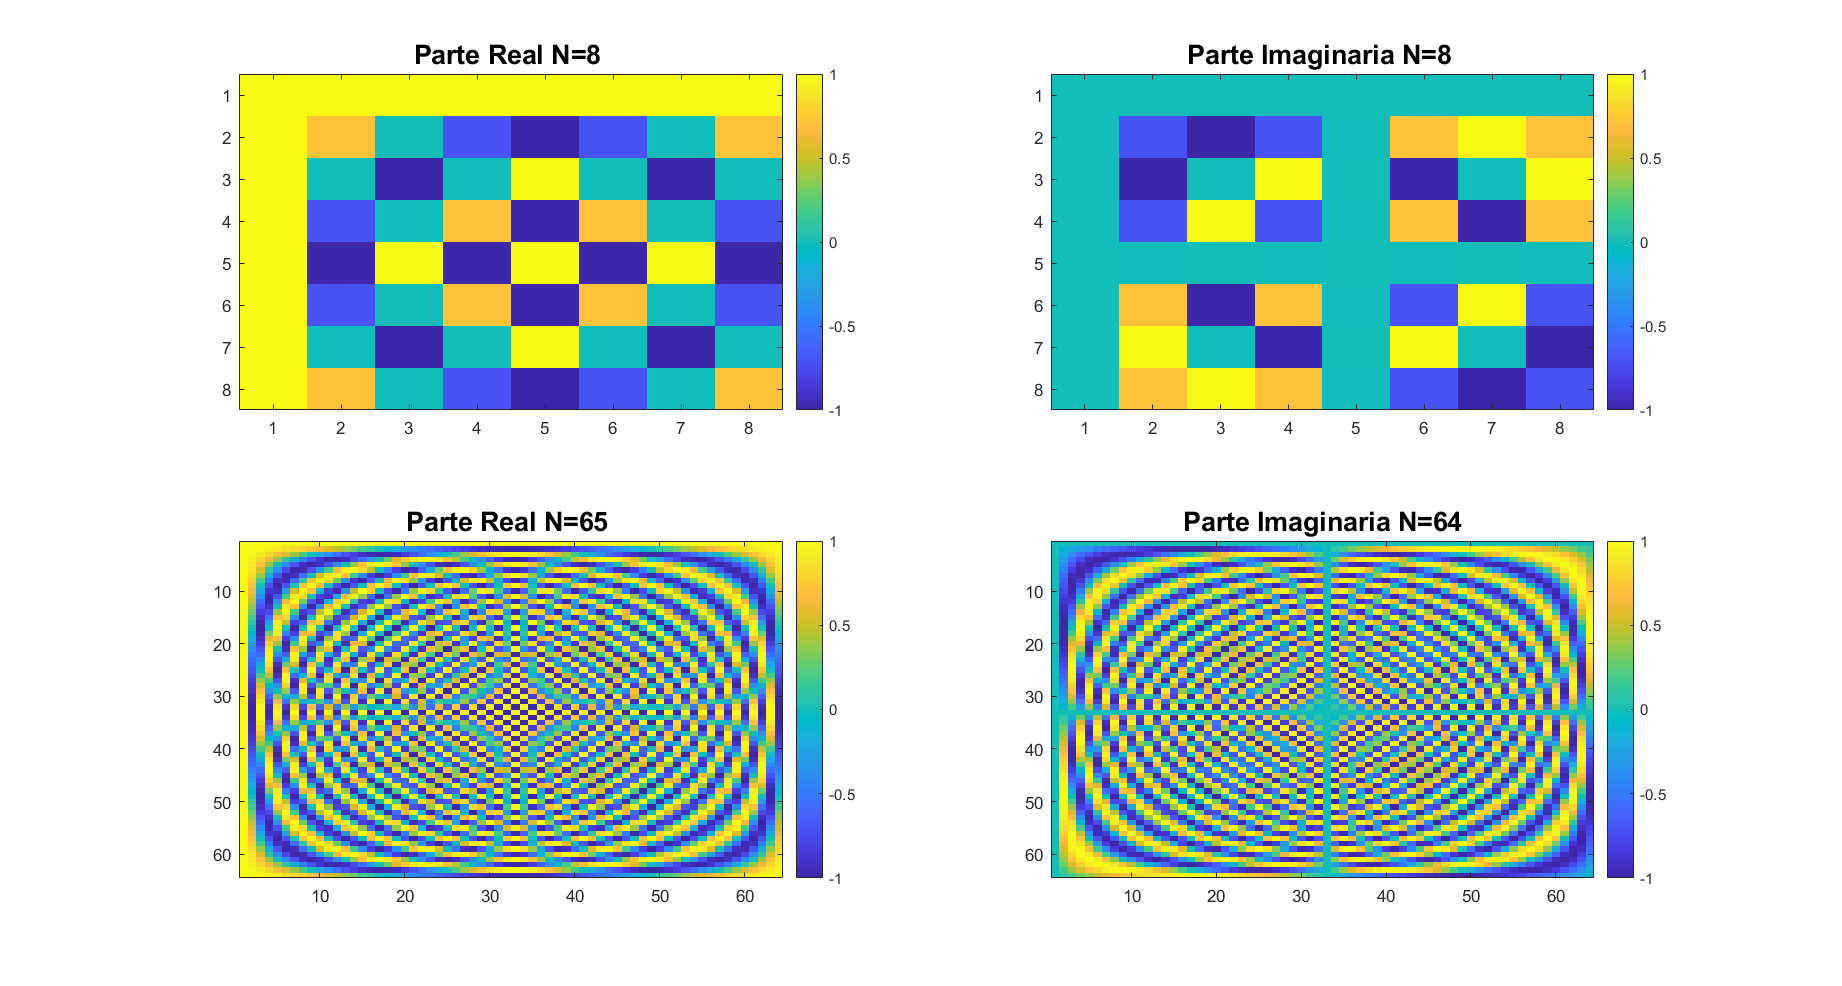
\includegraphics[width=1 \linewidth]{Figuras/V2.png}
\caption{Escala de colores para $genAmatrix$ de distintos tamaños.}
\label{V2}
\end{figure}
    
\item %3)--------------------------------------------------------------------------
El resultado de probar estas señales con la función diseñado $DFTmatrix$ y la función $fft$ de $MATLAB$ se muestra en la Figura \ref{V3}, que son equivalentes en magnitud. En la Figura \ref{V3b} se muestra el resultado de aplicarle a las funciones anterioremente descritas la señal $x_5 = cos(\omega t)$ con 5000 muestras.

\begin{figure}[H]
\centering
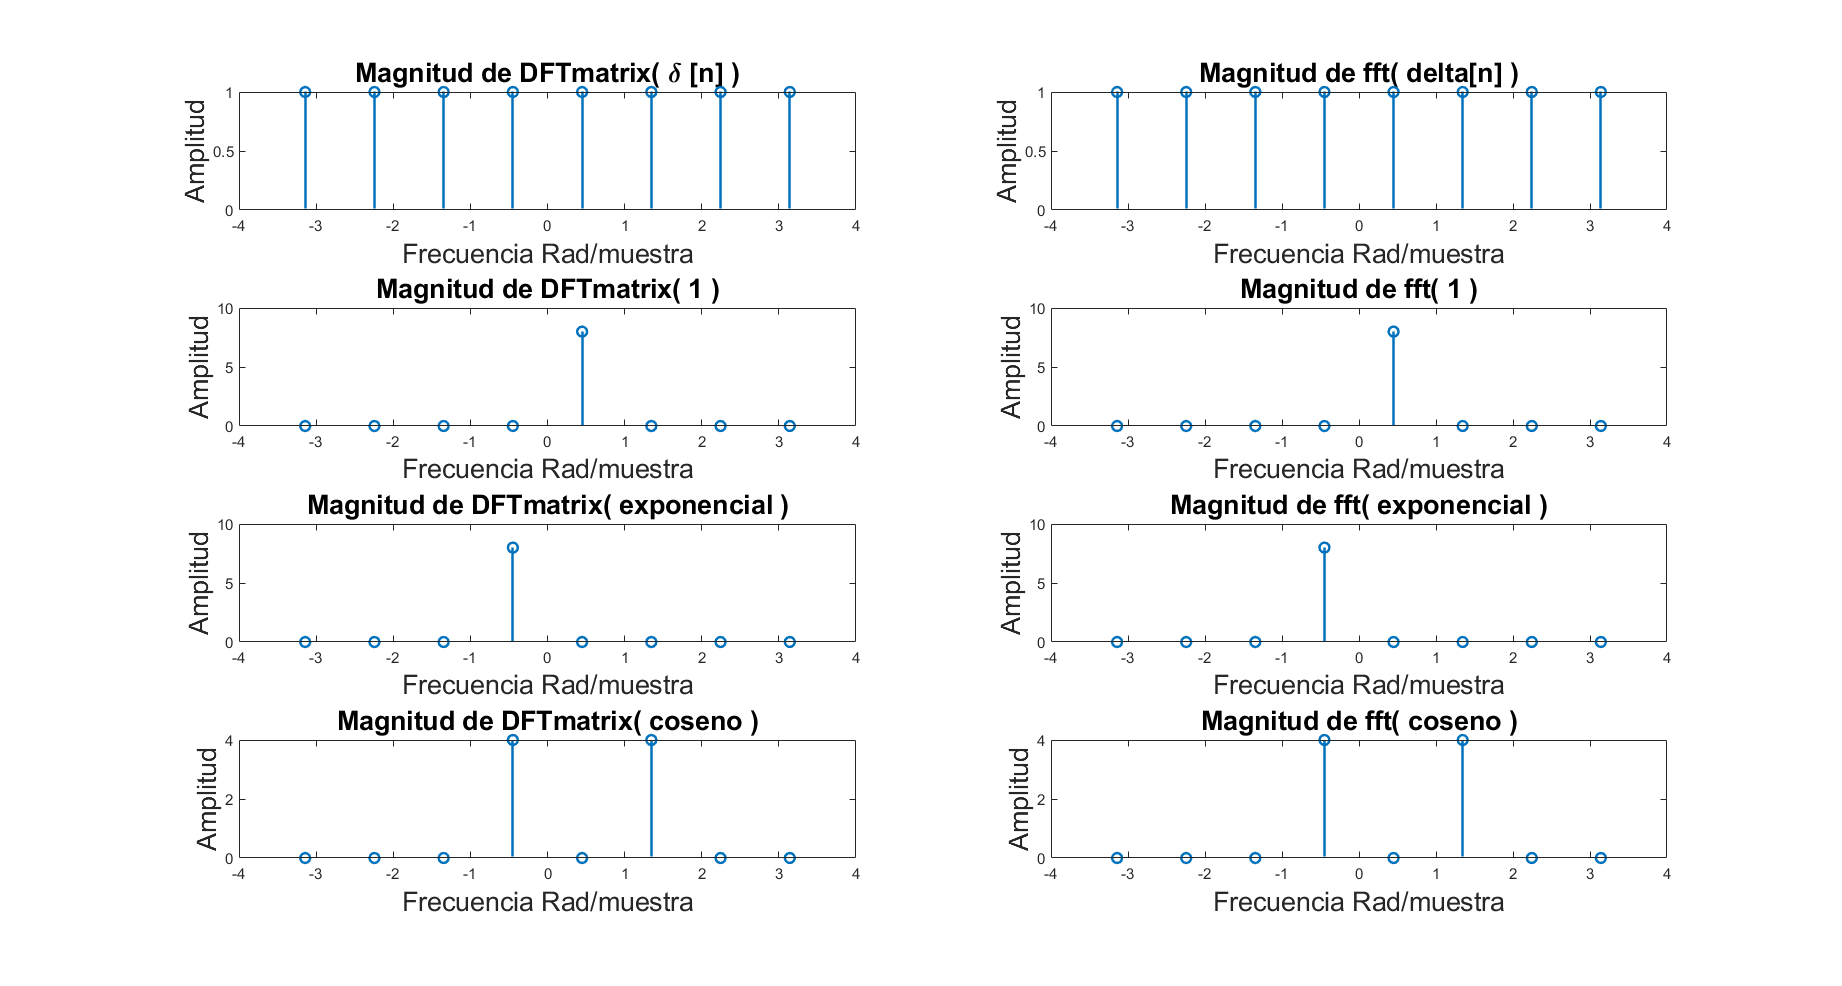
\includegraphics[width=1 \linewidth]{Figuras/V3.png}
\caption{Comparación con las distintas funciones.}
\label{V3}
\end{figure}
\begin{figure}[H]
\centering
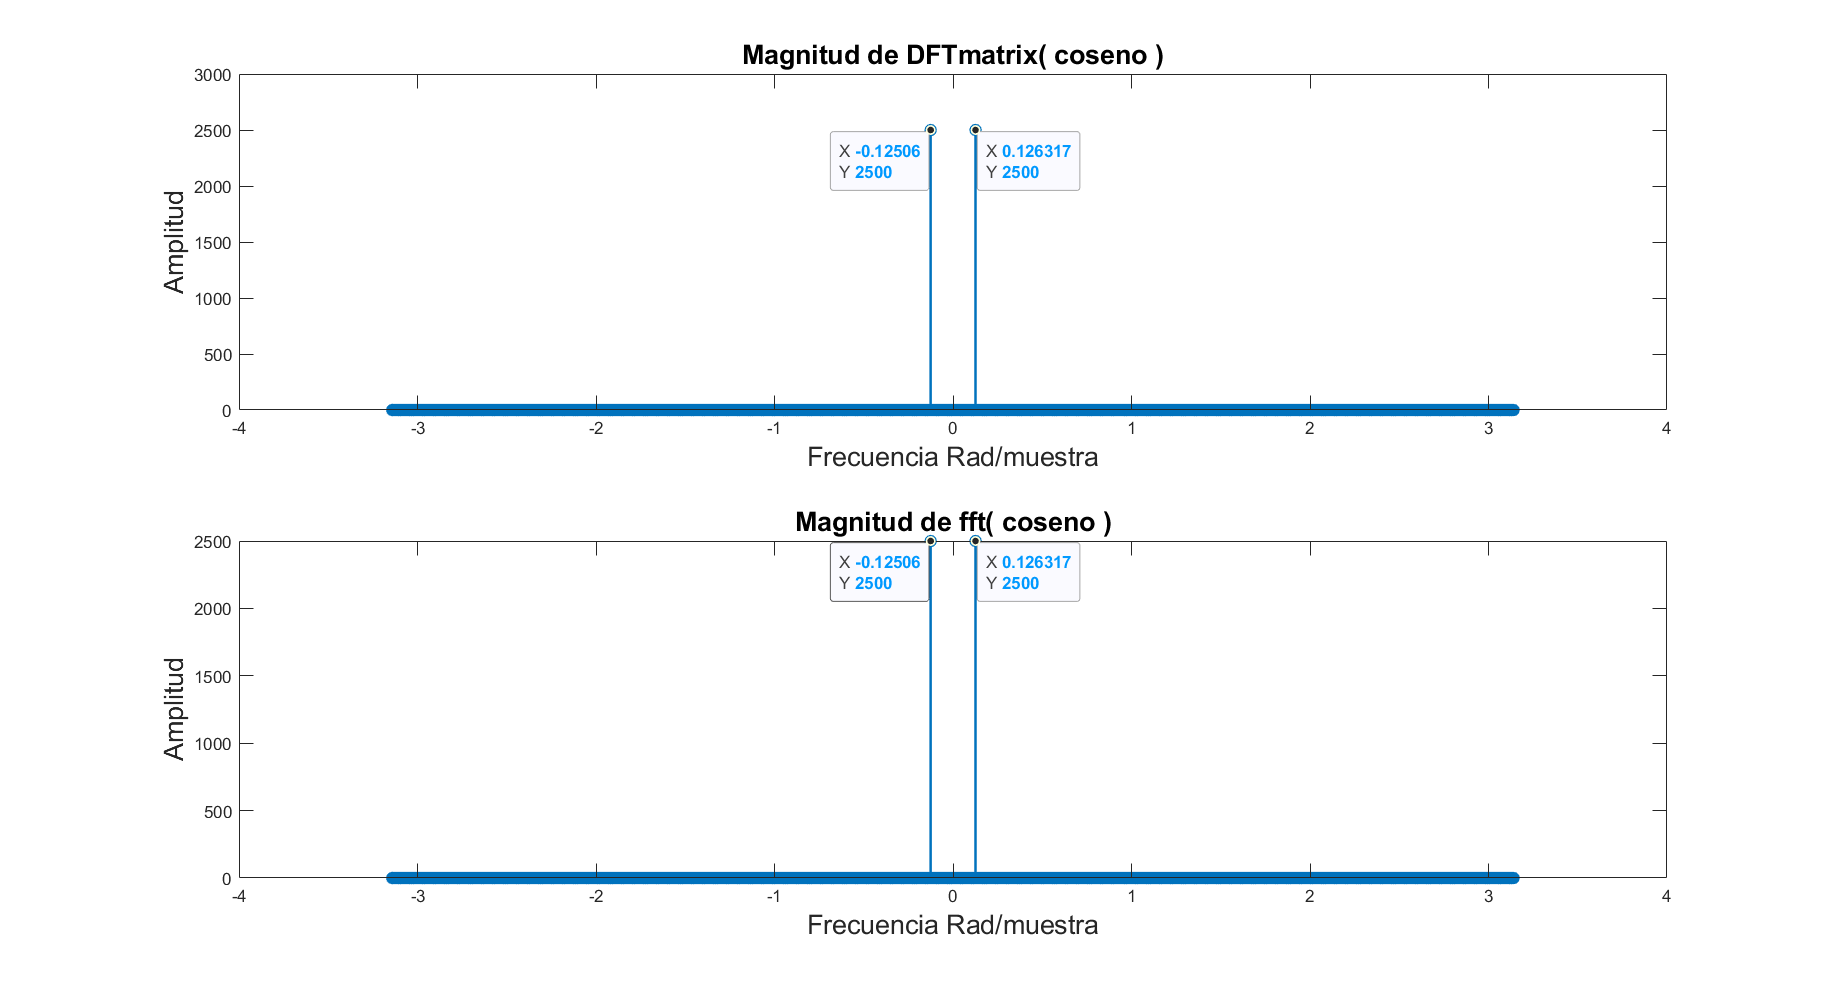
\includegraphics[width=1 \linewidth]{Figuras/V3b.png}
\caption{Comparación con las distintas funciones.}
\label{V3b}
\end{figure}
En la tabla \ref{tab:3} se muestra el error entre las función creadas y entre la función $DFTmatrix$ y $fft$, donde se mantiene el orden de magnitud para los errores al cambiar N, excepto para la señal $x_5$, debido al alto numero de muestras.
\begin{table}[H]
        \centering
        \begin{tabular}{|c|c|c|}
        \hline
            Señal     & MSE(DFTmatrix,fft) & MSE(DFTmatrix,DFTsum) \\ \hline
            $x_1[n]$ & 0  & 0 \\
            $x_2[n]$ & 3.6901e-30 &3.3671e-32\\
            $x_3[n]$ & 9.8474e-30 &2.9198e-32\\
            $x_4[n]$ & 3.0622e-30 &1.2749e-32\\
            $x_5$  &2.2216e-21 &2.1528e-21\\\hline
        \end{tabular}
        \caption{MSE entre Función $DFTsum$ y $fft$ de $MATLAB$}
        \label{tab:3}
\end{table}
    
    \item %4)--------------------------------------------------------------------------

Se miden los tiempos de comparación para la señal $x_5 = cos(\omega t)$ con 5000 muestras utilizando el siguiente script:
\begin{lstlisting}
fs=5000;
t=0:1/fs:1-1/fs;
x1=cos(2*pi*100*t);
f1 = @()DFTsum(x1);
f2 = @()DFTmatrix(x1);
t1_0 = timeit(f1);
t2_0 = timeit(f2);
\end{lstlisting}
Con lo que se obtienen los tiempos mostrados en la tabla \ref{tab:4}, donde se persive una mejora usando matrices en el calculo.
\begin{table}[H]
        \centering
        \begin{tabular}{|c|c|c|}
        \hline
            Señal     & Tiempo DFTsum s& Tiempo DFTmatrix s \\ \hline
            $x_5$  &5.67202599995000 &5.28868089995000\\\hline
        \end{tabular}
        \caption{Tiempo de ejecución para Función $DFTsum$ y $DFTmatrix$}
        \label{tab:4}
\end{table}
Se comparan los tiempos usando diferentes números de muestras N para la funcion $x_5 = cos(\omega t)$ utilizando el siguiente script de $MATLAB$:
\begin{lstlisting}
fs=5000;
t=0:1/fs:1-1/fs;
t1=zeros([1,50]);
t2=zeros([1,50]);
t3=zeros([1,50]);
x5=cos(2*pi*100*t);
i=1;
for N=100:100:5000
    f1 = @()DFTsum(x5(1:N));
    f2 = @()DFTmatrix(x5(1:N));
    f3 = @()fft(x5(1:N));
    f4 = @()dftmtx(N);
    t1(i) = timeit(f1);
    t2(i) = timeit(f2);
    t3(i) = timeit(f3);
    t4(i) = timeit(f4);
    i=i+1;
end
\end{lstlisting}
El grafico de los tiempos de ejecución para las diferentes funciones se muestra en la Figura \ref{V4}, donde se aprecia como el tiempo de ejecución tiene una curva exponencial para los métodos implementados DFTsum y DFTmatrix. Se aprecia como el tiempo de ejecución de la función $fft$ tiene tiempos más cortos, y con una curva logaritmica. Al apreciar los tiempo de la función $dftmtx$ de matlab se concluye que la creación de la matriz no influye de sobre manera en los tiempos de ejecución del algoritmo $DFTmatrix$.\\
Finalmente la función $fft$ es la más eficiente, se destaca que, en $MATLAB$ la función $DFTmatrix$ es más eficiente que la función $DFTsum$ por el uso de matrices, ya que el programa esta optimizado para las operaciones con estas. Por la forma de trabajar porciones de datos, la función $fft$ ocupa más recuersos de memoria.
\begin{figure}[H]
\centering
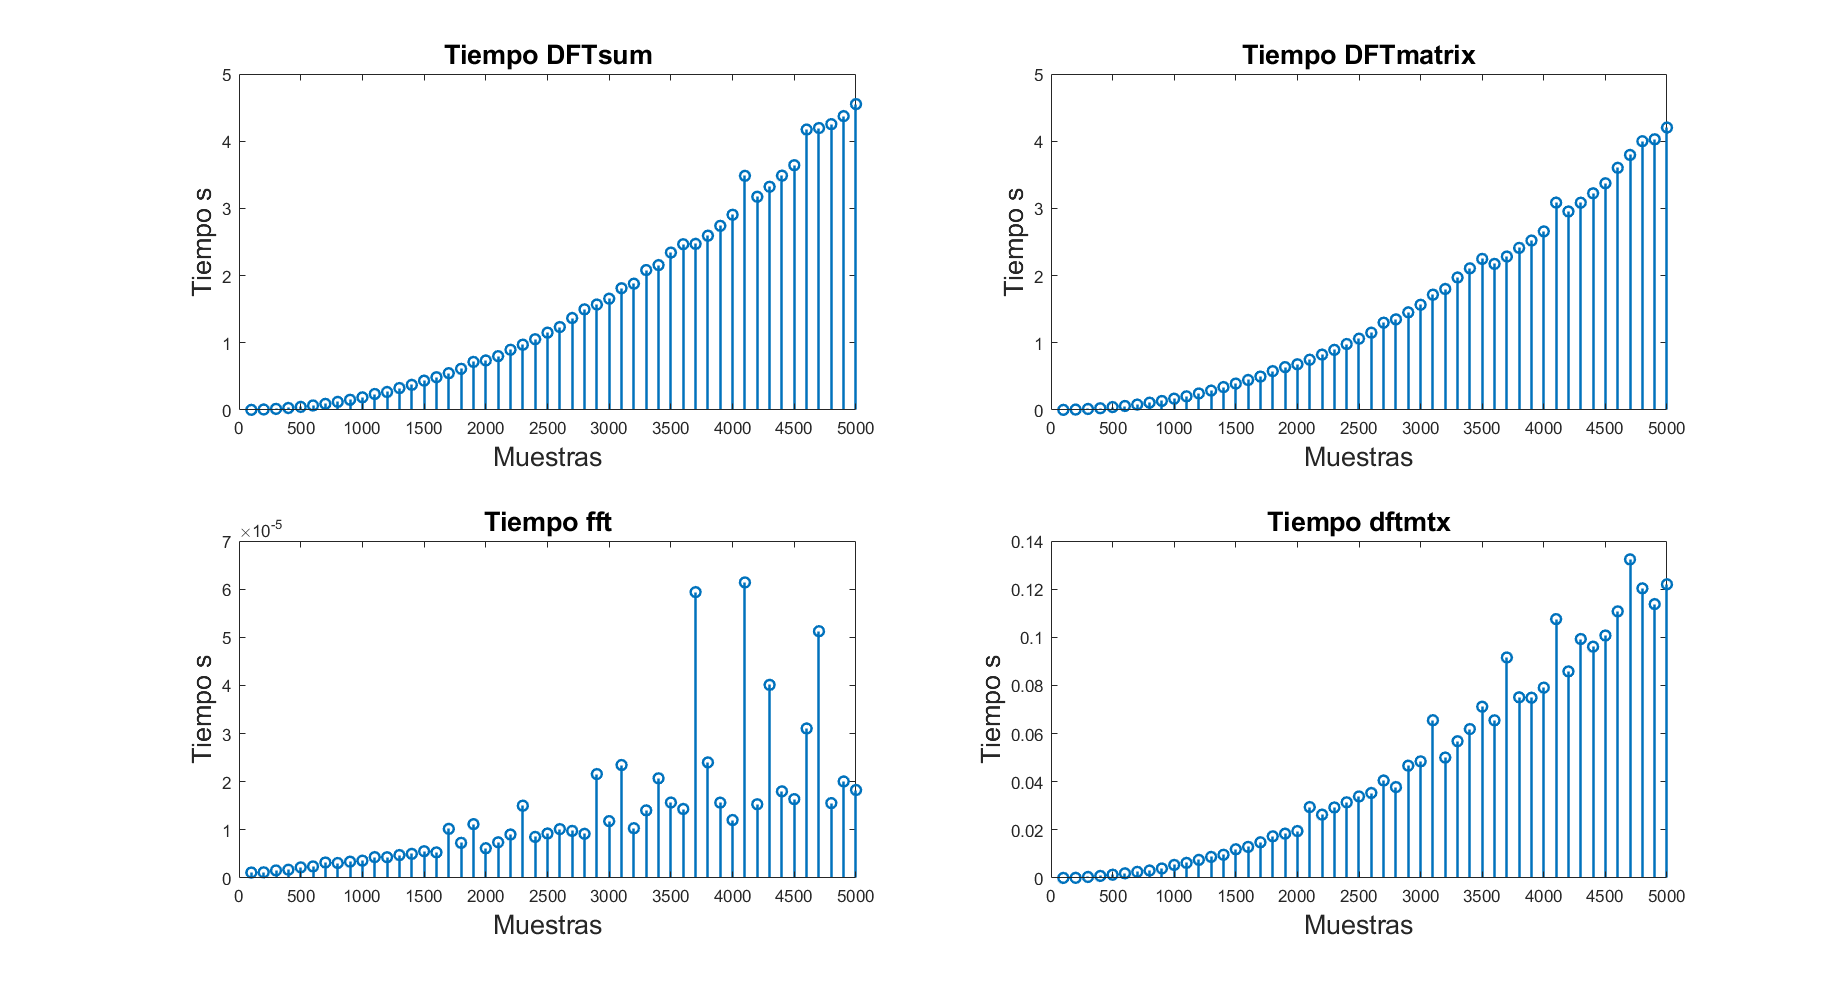
\includegraphics[width=1 \linewidth]{Figuras/V4.png}
\caption{Comparación con las distintas funciones.}
\label{V4}
\end{figure}
\end{enumerate}
%%%%%%%%%%%%%%%%%%%%%%%%%%%%%%%%%%%%%%%%%%%%%%%%%%%%%%%%%%%%%%%%%%%%%%%%%%%%%%%%%
%
%--VI. ALGORITMORADIX-2DE LAFFT-------------%
%
%%%%%%%%%%%%%%%%%%%%%%%%%%%%%%%%%%%%%%%%%%%%%%%%%%%%%%%%%%%%%%%%%%%%%%%%%%%%%%%%%
\section{Algoritmo Radix-2 de la FFT}
\begin{enumerate}[1)]
    \item %1)-------------------------------------------------------------------------%
    Se implementó la siguiente función para implementar la DFT con reducción de orden.
    \begin{lstlisting}
    function X=dftdc(x)
    x_par=zeros([1,ceil(length(x))*0.5]);
        for n=1:length(x)
            if mod(n,2)~=0
                x_par((n+1)/2)=x(n);
            end
        end
    x_impar=zeros([1,ceil(length(x))*0.5]);
        for n=1:length(x)
            if mod(n,2)==0
                x_impar(n/2)=x(n);
            end
        end
    X_par=DFTsum(x_par);
    X_impar=DFTsum(x_impar);
    k=0:length(X_impar)-1;
    Wnk=exp(-j*2*pi*k/length(x));
    X=[X_par+Wnk.*X_impar, X_par-Wnk.*X_impar];
    end
    \end{lstlisting}
    
    Se aplicó el algoritmo para las mismas señales que en VI-1, demostrando, en los gráficos de la figura \ref{fig:VI1} que se obtiene adecuadamente la dft de la señal.
    \begin{figure}[H]
        \centering
    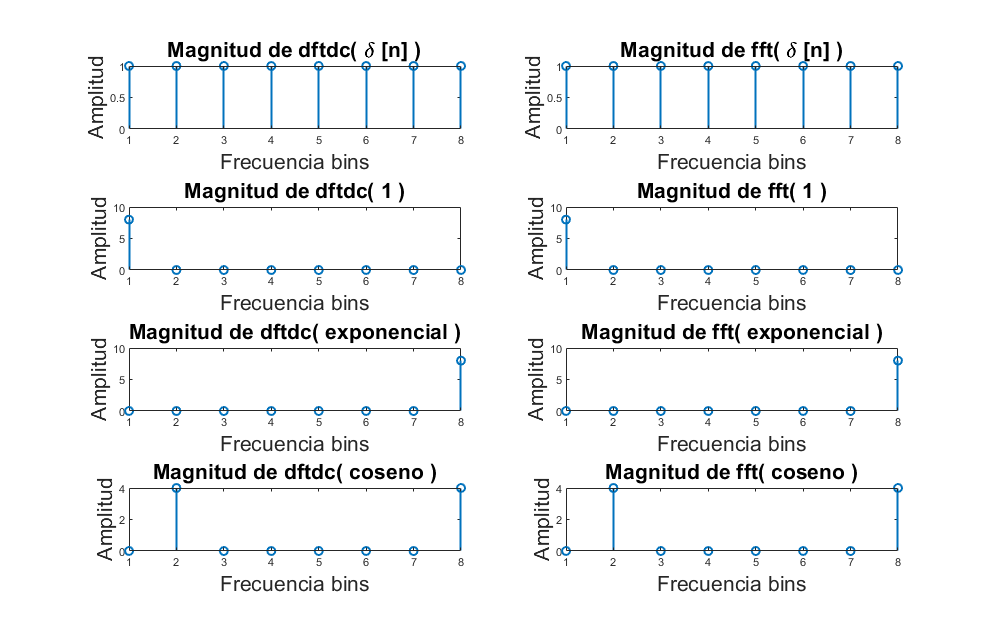
\includegraphics[width= \linewidth]{Figuras/VI1.png}
        \caption{Comparación entre fft y dftdc}
        \label{fig:VI1}
    \end{figure}
    
    Los tiempos de ejecución para ambas funciones con la señal $\delta(n)$ de ocho muestras se observan en la tabla \ref{tab:5}. Donde se observa que la $fft$ de MATLAB sigue siendo más rápida.
    \begin{table}[H]
        \centering
        \begin{tabular}{|c|c|c|}
        \hline
            Señal     & Tiempo DFTdc s& Tiempo fft s \\ \hline
            $x_5$  &2.368314411764706e-05 &7.550727772227772e-07\\\hline
        \end{tabular}
        \caption{Tiempo de ejecución para Función $DFTdc$ y $fft$ de MATLAB}
        \label{tab:5}
\end{table}
    
    \item %2)-------------------------------------------------------------------------%
    Se implementan las siguientes funciones, las cuales calculan la FFT de una señal para 8, 4 y 2 puntos respectivamente, en este caso, la función FFT8 llama a FFT4, y la función FFT4 llama a FFT2:
    \begin{lstlisting}
        function X = FFT8(x)
        Wn = exp(-1j*2*pi/8);
        X = zeros([1,8]);
        x0 = [x(1) x(3) x(5) x(7)];
        X0 = FFT4(x0);
        x1 = [x(2) x(4) x(6) x(8)];
        X1 = FFT4(x1);
            for k=1:4
                X(k) = X0(k)+Wn^(k-1)*X1(k);
                X(k+4) = X0(k)-Wn^(k-1)*X1(k);
            end
        end
        
        function X = FFT4(x)
        Wn = exp(-1j*2*pi/4);
        X = zeros([1,4]);
        x0 = [x(1) x(3)];
        X0 = FFT2(x0);
        x1 = [x(2) x(4)];
        X1 = FFT2(x1);
            for k=1:2
                X(k) = X0(k)+Wn^(k-1)*X1(k);
                X(k+2) = X0(k)-Wn^(k-1)*X1(k);
            end
        end
        
        function X = FFT2(x)
        X(1) = x(1)+x(2);
        X(2) = x(1)-x(2);
        end

    \end{lstlisting}
    Se graficaron las señales anteriores con FFT8, corroborando que las funciones implementadas calculan correctamente la dft. Los gráficos se muestran en la figura \ref{fig:VI2}
    \begin{figure}[H]
        \centering
        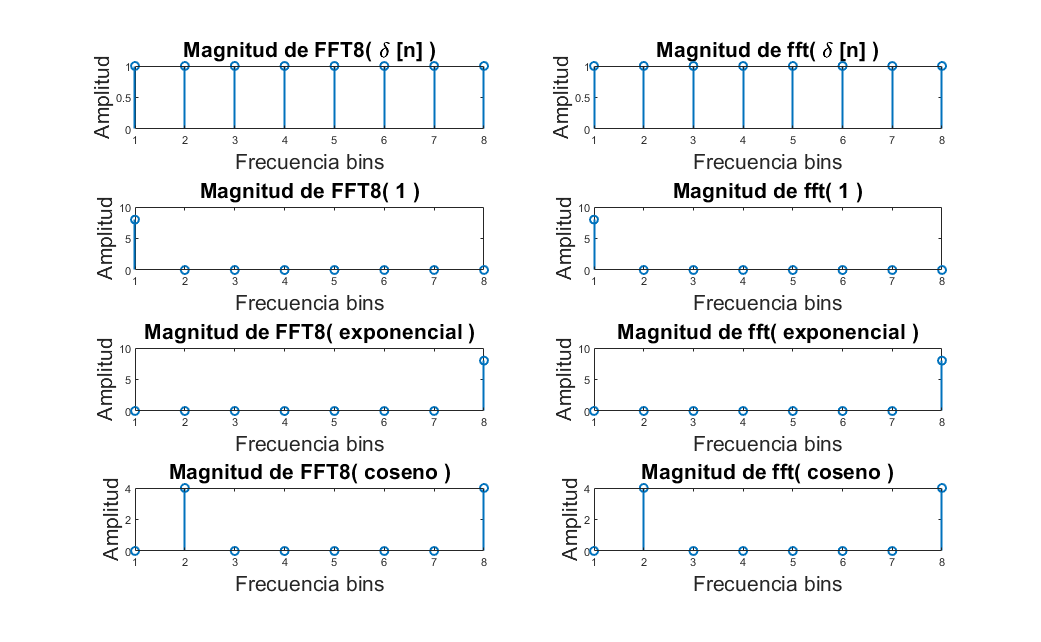
\includegraphics[width=\linewidth]{Figuras/VI2.png}
        \caption{Comparación entre fft y FFT8}
        \label{fig:VI2}
    \end{figure}
    El tiempo de procesamiento obtenido para el delta $\delta (n)$ de 8 muestras en este caso es de $1.303173888888889e-05$ s, siendo un poco mas leve que para la función del punto anterior, pero aún superior a la $fft()$ de MATLAB.
    \newpage
    \item %3)-------------------------------------------------------------------------%
    A partir de la lógica de las funciones anteriores, se implementa finalmente la función recursiva $fft\_stage(x)$, que obtiene la fft de la señal $x$.
    \begin{lstlisting}
        function X = fft_stage(x)
        if length(x) == 2
            X =FFT2(x);
        else
            x_par=zeros([1,ceil(length(x))*0.5]);
            for n=1:length(x)
                if mod(n,2)~=0
                    x_par((n+1)/2)=x(n);
                end
            end
            x_impar=zeros([1,ceil(length(x))*0.5]);
            for n=1:length(x)
                if mod(n,2)==0
                    x_impar(n/2)=x(n);
                end
            end
            X_par = fft_stage(x_par);
            X_impar = fft_stage(x_impar);
            
            k=0:length(X_impar)-1;
            Wnk=exp(-j*2*pi*k/length(x));
            X=[X_par+Wnk.*X_impar, X_par-Wnk.*X_impar];
        end
        end
    \end{lstlisting}
    Se comprobó tanto la dft calculada por la función $ff\_stage$ como la $fft$ de \textsc{matlab} para $256$ muestras de un coseno con frecuencia $100$. Se observa que la función $fft\_stage$ calcula la fft correctamente
    \begin{figure}[H]
        \centering
        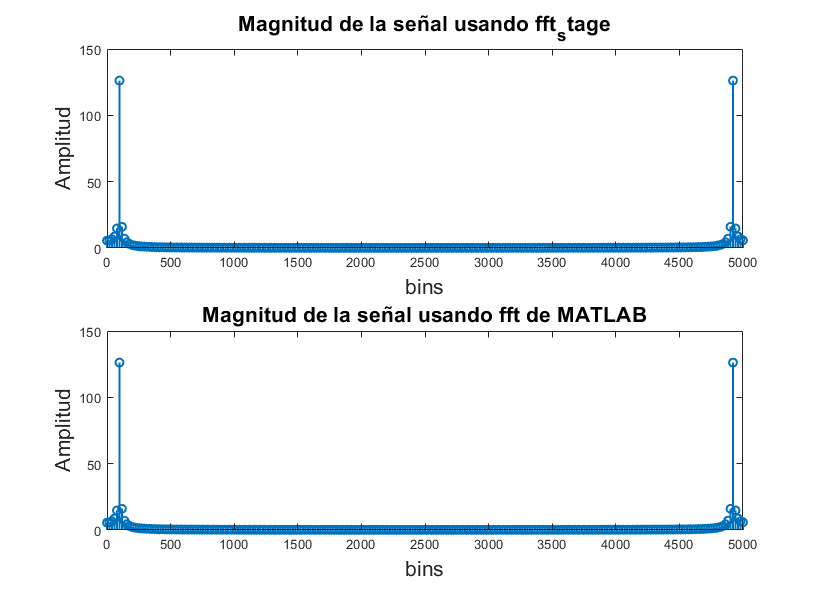
\includegraphics[width=\linewidth]{Figuras/VI3.png}
        \caption{Comparación entre algoritmos resultados de funciones $fft$ y $fft\_stage$}
        \label{fig:VI3}
    \end{figure}

Comparamos los tiempos de la función $fft\_stage$ generada y la función $fft$ de $MATLAB$ con el siguiente script:

\begin{lstlisting}
fs=5000;
t=linspace(0,3-1/fs,2^19);
x1=cos(2*pi*100*t);
i=1;
for k=10:19
    N = 2^k;
    f1 = @()fft_stage(x1(1:N));
    f2 = @()fft(x1(1:N));
    t1(i) = timeit(f1);
    t2(i) = timeit(f2);
    i=i+1;
end
\end{lstlisting}

Los resultados de esto se muestran en la Figura \ref{VI4}, donde las muestras N = [0, 1, ..., 10] corresponden a n = [$2^{10}$, $2^{11}$, ... $2^{19}$]. Se aprecia que los tiempos de ejecución de ambas funciones escalan de igual forma. Los tiempos la función $fft\_stage$ son buenos respecto a las otras funciones que se implementaron, pero la función $fft$ sigue siendo más eficiente.

\begin{figure}[H]
\centering
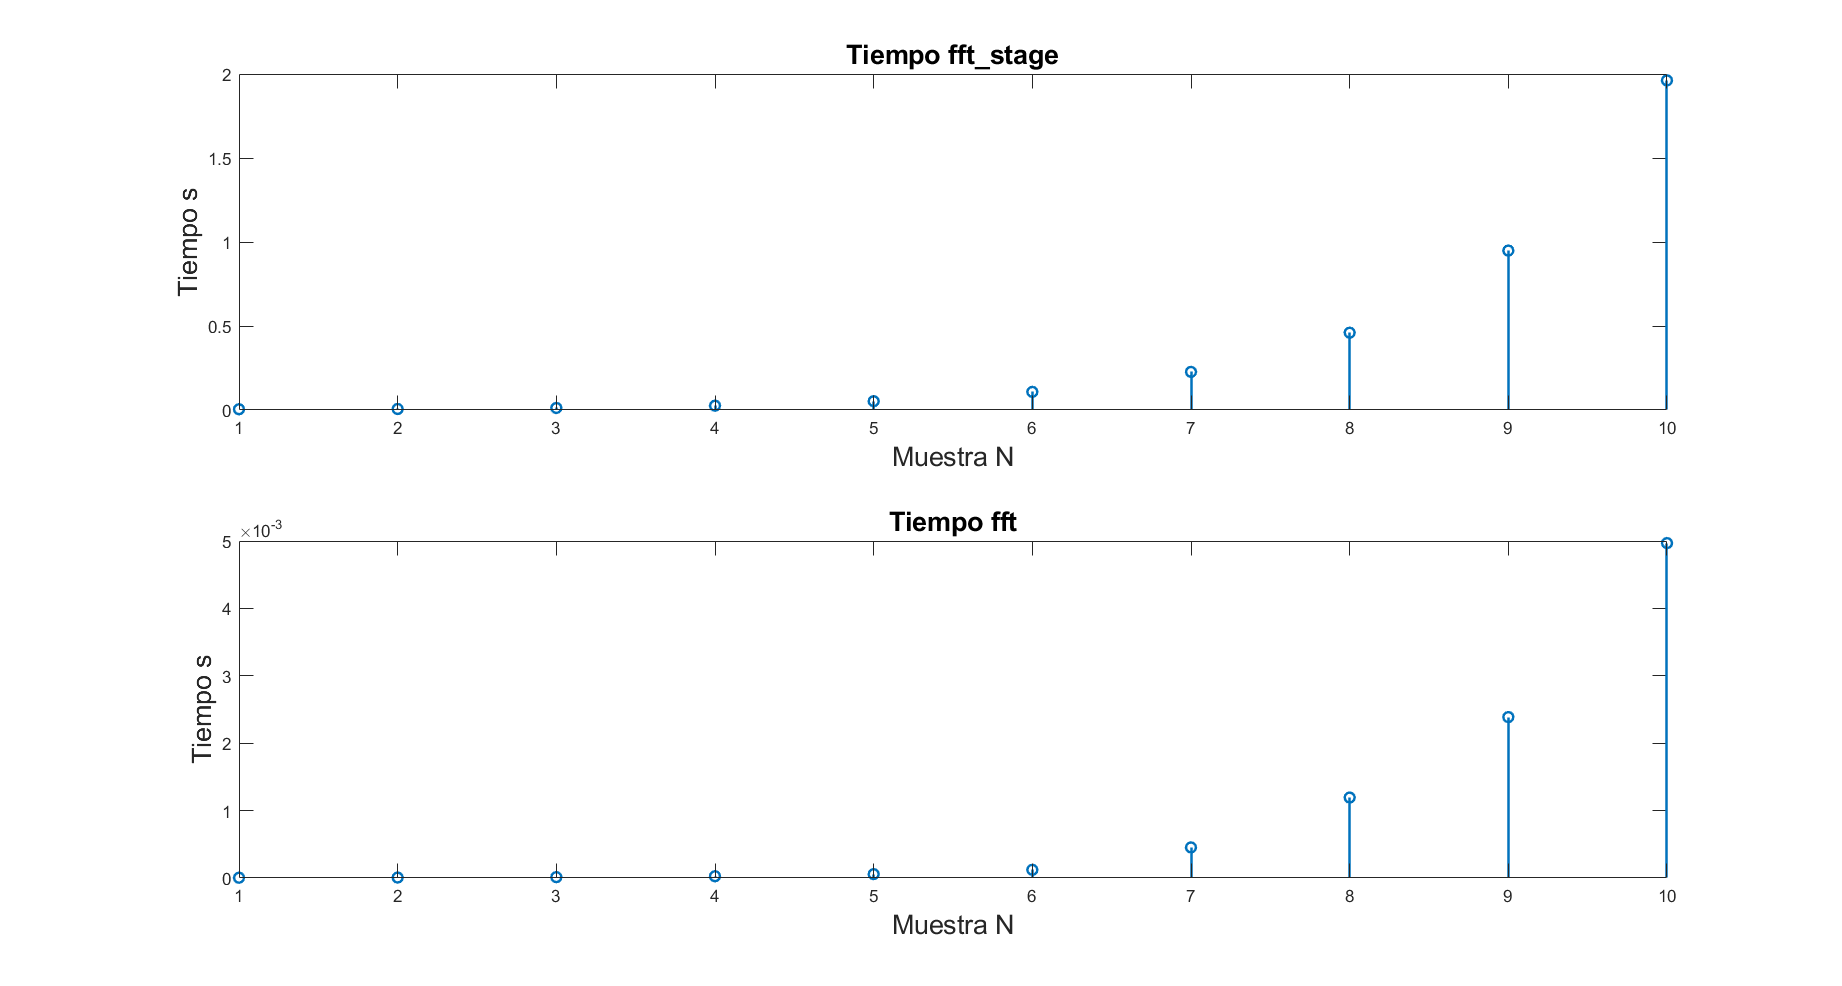
\includegraphics[width=\linewidth]{Figuras/VI4.png}
\caption{Comparación entre tiempos resultados de funciones $fft$ y $fft\_stage$}
\label{VI4}
\end{figure}
\end{enumerate}
%%%%%%%%%%%%%%%%%%%%%%%%%%%%%%%%%%%%%%%%%%%%%%%%%%%%%%%%%%%%%%%%%%%%%%%%%%%%%%%%%
%
%--VII. IMPLEMENTACI ́ON EN S-FUNCTIONS: ALGORITMO DEGOERTZEL-------------%
%
%%%%%%%%%%%%%%%%%%%%%%%%%%%%%%%%%%%%%%%%%%%%%%%%%%%%%%%%%%%%%%%%%%%%%%%%%%%%%%%%%
\section{Implementación en S-Functions: Algoritmo de Goertzel}
\begin{enumerate}[1)]
    \item %1)-------------------------------------------------------------------------%
    Se creó la siguiente función (ejecutada una sola vez) para inicializar los parámetros del filtro Goertzel:
    \begin{lstlisting}[language=C]
        static void initGoertzel(goertzelState_t *state, uint64_t kFrequency)
        {
          double omega = (2*M_PI*kFrequency/GOERTZEL_N);
          state->samplesCounter = 0;
          state->cosW = cos(omega);
          state->sinW = sin(omega);
          state->A1= -2*cos(omega);
          state->outputs[0] = 0.0;
          state->outputs[1] = 0.0;
          state->outputs[2] = 0.0;
          state->binReal=0;
          state->binImag=0;
          state->binMag=0;
        	return;
        }
    \end{lstlisting}
    Luego, la siguiente función permite filtrar la señal según la formula de Goertzel, y devuelve el valor del BIN requerido luego de N muestras:
    \begin{lstlisting}[language=C]
        static double computeGoertzel(goertzelState_t *state, double filterInput)
        {
        state->outputs[2]=state->outputs[1];
        state->outputs[1]=state->outputs[0];
        state->outputs[0]=filterInput+(2*state->cosW*state->outputs[1])-(state->outputs[2]);
        (state->samplesCounter)+=1;
        
        if(state->samplesCounter==GOERTZEL_N)
        {
          state->binReal=state->cosW*state->outputs[1]-state->outputs[2];
          state->binImag=state->sinW*state->outputs[1];
          state->binMag=sqrt(state->binReal*state->binReal+state->binImag*state->binImag);
          resetGoertzel(state);
        }
        return state->binMag;
        }
    \end{lstlisting}
    Para comprobar el funcionamiento del programa, se miden los bins $8,9,10$ de la transformada de Fourier de las primeras $256$ muestras, lo que se observa en la figura
    \begin{figure}[H]
        \centering
        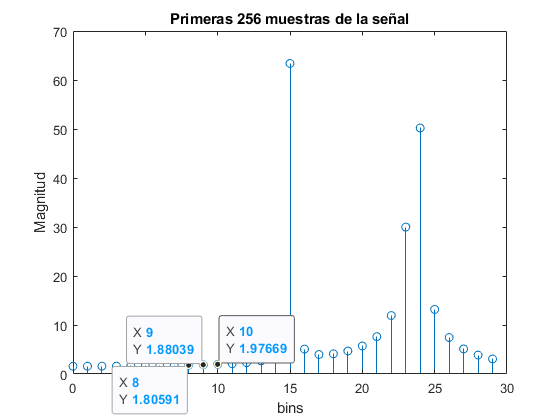
\includegraphics[width=0.8 \linewidth]{Figuras/VII1.png}
        \caption{Bins del primer frame de la señal}
        \label{fig:VII1}
    \end{figure}
    Luego, se comparan con la salida luego de N muestras de la S-Function, seleccionando los bins $8, 9, 10$. Donde se observa que los valores obtenidos corresponden efectivamente a las magnitudes del bin.
    \begin{figure} [H]
        \centering
        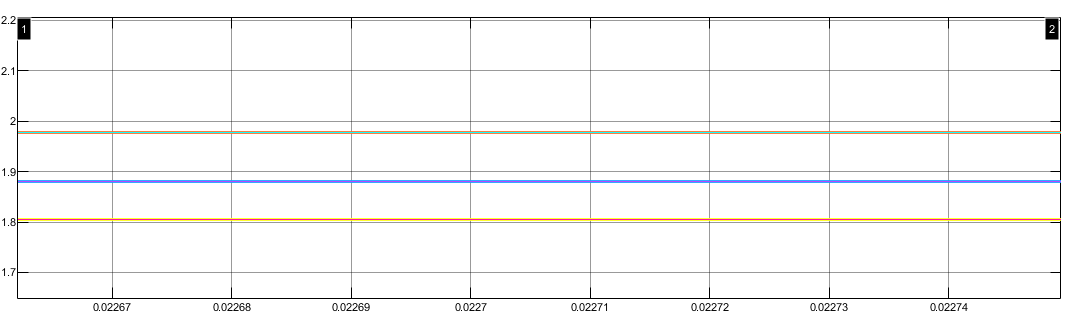
\includegraphics[width=0.8 \linewidth]{Figuras/VII1b.png}
        \caption{Bins obtenidos en la salida, 8 en amarillo, 9 en azul y 10 en marrón}
        \label{fig:VII1b}
    \end{figure}
    \item %2)-------------------------------------------------------------------------%
    Para elegir los bins, se calculan transformadas de Fourier de 256 puntos en distintos momentos de la señal, correspondiente a distintos tonos. Luego se eligen los dos bins con mayor magnitud (Para identificar cada tono más fácilmente, se utilizó la señal \textit{dtmfSequenceSpaced\_16\_16.wav}). Obteniéndose la siguiente tabla:
    \begin{table}[H]
        \centering
        \begin{tabular}{|c|c|c|}
        \hline
        Primer sample & bin 1 & bin 2 \\
        \hline
        0 & 15 & 24 \\
        4000 & 15 & 21 \\
        8000 & 11 & 24 \\
        11000 & 11 & 19 \\
        13000 & 12 & 19 \\
        17000 & 14 & 24 \\
        \hline
        \end{tabular}
        \caption{Bins obtenidos}
        \label{tab:tabla6}
    \end{table}
    
    De esta forma, los 7 bins obtenidos son $11, 12, 14, 15, 19, 21, 24$
    
    Luego, se ejecuta el código a cada uno de estos bins, creando 7 estructuras de tipo \textit{goertzelState\_t}. Y aplicando las funciones a cada una de ellas.
    \begin{lstlisting}[language=C]
        /* Inicializacion */
          initGoertzel( &gGoertzelState1 , GOERTZEL1_K_BIN );
          initGoertzel( &gGoertzelState2 , GOERTZEL2_K_BIN );
          initGoertzel( &gGoertzelState3 , GOERTZEL3_K_BIN );
          initGoertzel( &gGoertzelState4 , GOERTZEL4_K_BIN );
          initGoertzel( &gGoertzelState5 , GOERTZEL5_K_BIN );
          initGoertzel( &gGoertzelState6 , GOERTZEL6_K_BIN );
          initGoertzel( &gGoertzelState7 , GOERTZEL7_K_BIN );
    \end{lstlisting}
    \begin{lstlisting}[language=C]
    /* Funcion principal */
        void goertzelFunction(double input1,
				double *output1,
				double *output2,
				double *output3,
				double *output4,
				double *output5,
				double *output6,
				double *output7
				)
        {
          *output1 = computeGoertzel(&gGoertzelState1 , input1);
          *output2 = computeGoertzel(&gGoertzelState2 , input1);
          *output3 = computeGoertzel(&gGoertzelState3 , input1);
          *output4 = computeGoertzel(&gGoertzelState4 , input1);
          *output5 = computeGoertzel(&gGoertzelState5 , input1);
          *output6 = computeGoertzel(&gGoertzelState6 , input1);
          *output7 = computeGoertzel(&gGoertzelState7 , input1);
        }
    \end{lstlisting}
    
    
    El resultado en la salida de la s-Function es mandado a \textsc{MATLAB} mediante la función \textit{toWorkspace}.
    
    Luego, cada para cada bin $i$ de $i=1:7$, se gráfica según el comando:
    
    \begin{lstlisting}
        bar(out.tout,out.bins(:,i))
    \end{lstlisting}
    
    Los gráficos obtenidos se muestran en la figura \ref{fig:VII2}, donde se comprueba que en cada momento solo hay dos bins en alto, (correspondientes a los valores de DTMF del tono pulsado).
    \begin{figure}[H]
        \centering
        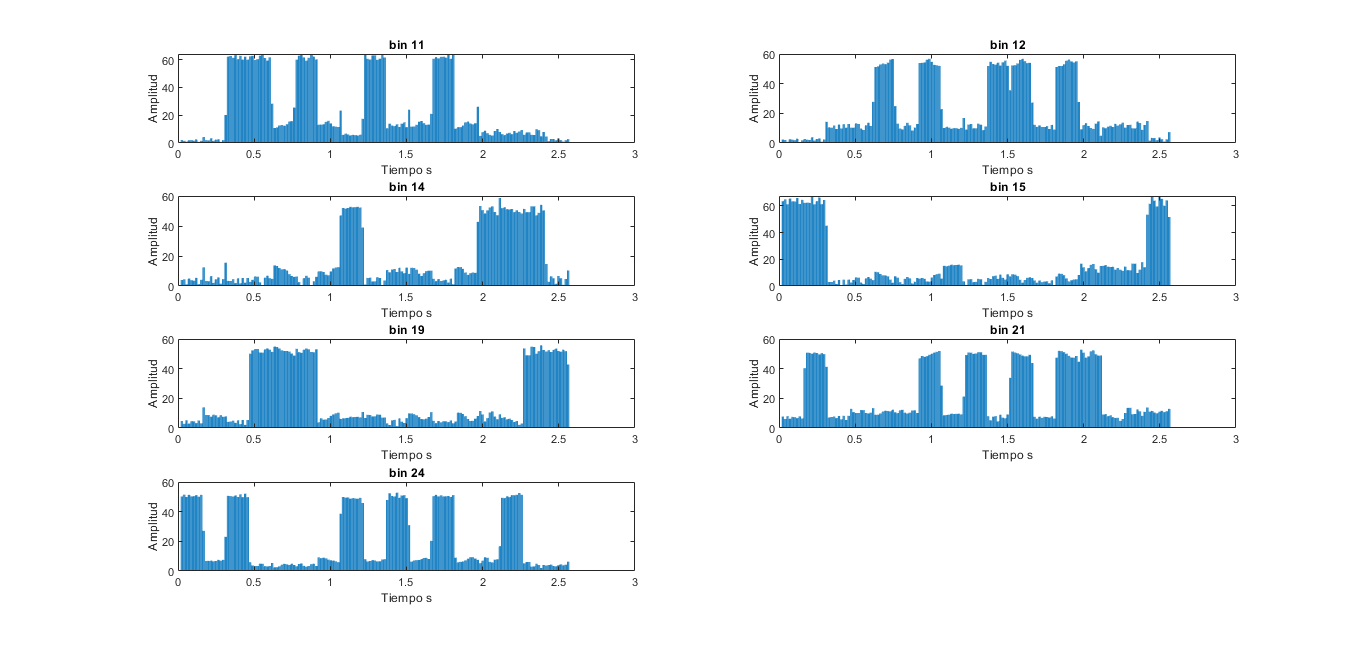
\includegraphics[width=\linewidth]{Figuras/VII2.png}
        \caption{coeficientes de salida para los 7 bins elegidos}
        \label{fig:VII2}
    \end{figure}
    De la secuencia decodificada del informe anterior se puede extraer que los bins corresponden a lo siguiente:
    \begin{table}[H]
        \centering
        \begin{tabular}{|c|c|}
        \hline
         Bin & Coordenada \\
         \hline
         11  & Primera fila \\ 
         12  & Segunda fila \\ 
         14  & Tercera fila \\ 
         15  & Cuarta fila \\ 
         19  & Primera columna \\ 
         21  & Segunda columna \\ 
         24  & Tercera columna \\
         \hline
        \end{tabular}
        \caption{Coordenadas del bin}
        \label{tab:bins}
    \end{table}
    Luego, de DTMF, a partir de la tabla \ref{tab:phone} y los graficos de la figura \ref{fig:VII2}, se corrobora que la secuencia es efectivamente $\#031415926535897*$.
    \begin{table}[H]
        \centering
        \begin{tabular}{|c|c|c|}
        \hline
        1 & 2 & 3 \\\hline
        4 & 5 & 6 \\\hline
        7 & 8 & 9 \\\hline
        * & 0 & \# \\
        \hline
        \end{tabular}
        \caption{Coordenadas numéricas}
        \label{tab:phone}
    \end{table}
\end{enumerate}

\end{document}
